%% ****** Start of file template.aps ****** % measurement
%%
%%
%%   This file is part of the APS files in the REVTeX 4 distribution.
%%   Version 4.0 of REVTeX, August 2001
%%
%%
%%   Copyright (c) 2001 The American Physical Society.
%%
%%   See the REVTeX 4 README file for restrictions and more information.
%%
%
% This is a template for producing manuscripts for use with REVTEX 4.0
% Copy this file to another name and then work on that file.
% That way, you always have this original template file to use.
%
% Group addresses by affiliation; use superscriptaddress for long
% author lists, or if there are many overlapping affiliations.
% For Phys. Rev. appearance, change preprint to twocolumn.
% Choose pra, prb, prc, prd, pre, prl, prstab, or rmp for journal
%  Add 'draft' option to mark overfull boxes with black boxes
%  Add 'showpacs' option to make PACS codes appear


\documentclass[11pt]{article}
\pdfoutput=1
\usepackage{amsmath}
\usepackage{amssymb}
\usepackage{mathtools}
%\usepackage{cite}
\usepackage{graphicx,bbm,mathrsfs}
\usepackage{nicefrac}
\usepackage{bbm}
\usepackage{geometry}
\usepackage{subdepth}
\geometry{a4paper}

\usepackage{jheppub}
%\usepackage{natbib}

\usepackage{dcolumn}   % needed for some tables
\usepackage{bm}        % for math
\usepackage{graphicx,mathrsfs}
\usepackage{nicefrac}
\usepackage{multirow}
\usepackage{color}
%\usepackage{bbm}

\usepackage[nomargin,inline,marginclue,draft]{fixme}
\fxsetup{theme=color}

\def\ie{{\it i.e.}}
\def\eg{{\it e.g.}}
\newcommand{\be}{\begin{equation}}
\newcommand{\ee}{\end{equation}}
\newcommand{\bea}{\begin{eqnarray}}
\newcommand{\eea}{\end{eqnarray}}
\renewcommand{\O}{\mathcal O}
\newcommand{\tr}{\operatorname{tr}}

\renewcommand{\d}{\mathbf{d}}

\usepackage{wasysym}


\renewcommand{\arraystretch}{1.2} % space between table rows


% avoids incorrect hyphenation, added Nov/08 by SSR

\makeatletter
\g@addto@macro\bfseries{\boldmath}
\makeatother

\newcommand{\specialcell}[2][c]{%
  \begin{tabular}[#1]{@{}c@{}}#2\end{tabular}}


%==================================================================
\begin{document}


\vspace*{30mm}

\begin{center}
{\LARGE \bf The Simplified Likelihood Framework
}
\par\vspace*{20mm}\par

{\large \bf Andy~Buckley$^{\,a}$, Matthew~Citron$^{\,b}$,  Sylvain~Fichet$^{\,c}$, Sabine~Kraml$^{\,d}$, Wolfgang~Waltenberger$^{\,e}$, Nicholas~Wardle$^{\,f}$}

\bigskip

{\em $^a$ School of Physics \& Astronomy, University of Glasgow, Glasgow, Scotland, UK}
\\
{\em $^b$ University of California, Santa Barbara, California, USA}
\\
{\em $^c$ ICTP-SAIFR \& IFT-UNESP, R. Dr. Bento Teobaldo Ferraz 271, S\~ao Paulo, Brazil}
\\
{\em $^d$ Laboratoire de Physique Subatomique et de Cosmologie, Universit\'e Grenoble-Alpes, CNRS/IN2P3, Grenoble, France  }
\\
{\em $^e$ }
\\
{\em $^f$ Imperial College London, South Kensington, London, UK }
\vspace*{5mm}



\vspace*{15mm}

{  \bf  Abstract }

\end{center}
\vspace*{1mm}




\noindent
\begin{abstract}

We present the Simplified Likelihood framework, a systematic approximation scheme  for experimental likelihoods such as those originating from LHC experiments. This framework  can be used  to simplify data analyses and to transmit realistic experimental likelihoods to the community.
We present an efficient method to compute the parameters of the simplified likelihood  from Monte Carlo simulations. The approach is validated using a realistic LHC-like toy search. \ldots




\end{abstract}

%\vspace{5.2cm }
%\noindent
%{\em E-mail:\\
%philippe.brax@ipht.fr \\ sylvain@ift.unesp.br\\ guillaume.pignol@lpsc.in2p3.fr
%\\
%}



\noindent
\newpage




\section{Introduction}


Scientific observations of the real world are by nature imperfect in the sense that they always contain some amount of
 uncertainty unrelated to data, the \textit{systematic}   uncertainty. Identifying, measuring and modeling all the sources of systematic uncertainty is an important part of running a scientific experiment. A thorough treatment of such uncertainties is especially important in exploratory fields like Particle Physics and Cosmology. In these fields of research,  %where one often searches for a small unexpected signal hidden in a large background.
today's experiments  can be of large scale and can contain a huge number of these  uncertainties. For instance in the case of the Large Hadron Collider (LHC) experiments, the experimental likelihood likelihood functions used in standard model measurements and searches for new physics can contain several thousands of systematic uncertainties.

Although sources of systematic uncertainty can be numerous and of very different nature, a general feature they share is that they are almost always independent of each other. This property of independence between the systematic uncertainties has profound consequences, and, as we will discuss soon, is the reason why the approach presented in this work is so efficient. Namely, independence of the uncertainties can be used in order to drastically simplify the experimental likelihood function, to the price of an often-negligible error that will be discussed at length in this paper.

The \textit{Simplified Likelihood} framework we present in this paper is a well-defined approximation scheme for experimental likelihoods. It can be used to simplify subsequent experimental analyses, to allow a uniform statistical treatment of published search-analysis data, and to ease the transmission of results between an experiment and the scientific community.
We build on the proposals for approximating likelihoods recently suggested in Refs.~\cite{Fichet:2016gvx,SL_note}, in which promising preliminary results have been shown.

In the context of the LHC, communicating the full experimental likelihoods via the \texttt{RooFit/Roostats} software framework~\cite{Verkerke:2003ir,Moneta:2010pm} has been suggested in Refs.~\cite{Kraml:2012sg,Boudjema:2013qla}. The presentation method we propose in this paper is complementary in that it is technically straightforward to carry out, without relying on any
particular software package. Additionally, the proposal of presenting LHC results decoupled from systematic uncertainties has been pursued in Ref.~\cite{Cranmer:2013hia} in the context of theoretical errors on Higgs cross-sections. For Higgs cross-sections and decays, the combined covariance of the Higgs theoretical uncertainties consistent with the simplified likelihood framework presented here has been determined in Ref.~\cite{Arbey:2016kqi}.

In this paper we unify and extend the initial proposals of Refs.~\cite{Fichet:2016gvx,SL_note}, and thoroughly test the accuracy of the approximations using simulated LHC searches for new phenomena.
Compared to Refs.~\cite{Fichet:2016gvx,SL_note}, an important progress accomplished is that we have been able to rigorously include asymmetries in the combined uncertainties, which is useful in order to avoid inconsistencies such as a negative event yield. Technically this is done by taking into account the next-to-leading term in the limit given by an appropriate version of the Central Limit Theorem (CLT).

The paper is organized as follows. As summary of the main results is given in Section~\ref{se:EL_SL}. Section~\ref{se:SL_theory} contains the formal material, including
an interesting result about the next-to-leading term of the CLT and the derivation of the simplified likelihood formula. Section~\ref{se:SL_LHC} contains details about LHC likelihoods. A first validation of the simplified likelihood framework is done in Section~\ref{se:toy_search}.

%The CLT is often used in its asymptotic limit where the distribution becomes exactly normal. In the context of the simplified framework, however, there is a number of reasons to keep the next-to-leading
% term in the large-$N$ expansion of the CLT. The next-to-leading term encodes skewness: it is the main information about asymmetry of the distribution. The asymmetry of the distribution can be a relevant feature for the analyses hence it is safer to keep this information. Moreover a normal distribution has a support on $\mathbf{R}$, while quantities like event yields are defined on $\mathbf{R}^+$. A normal distribution of the nuisance parameter can give inconsistencies, such as a negative yield. This is a problem both conceptually and at the level of the concrete analyses. This happens because the pure Gaussian approximation is too rough.
% To have an asymmetric support such as $\mathbf{R}^+$,  the distribution must be asymmetric, hence the skew has to be taken into account.


\section{From the Experimental Likelihood to the Simplified Likelihood}
\label{se:EL_SL}

This section introduces the formalism, presents the main theoretical results and an efficient Monte-Carlo based calculation method. We will focus on the typical experimental likelihood used in searches for new phenomena at particle physics experiments. However we stress that the simplified likelihood approach can be easily generalized to other physics contexts.
The data collected in particle physics usually originate from random (quantum) processes, and have thus have an intrinsic \textit{statistical} uncertainty--which vanishes in the limit of large data sets. Our interest rather lies in the \textit{systematic} uncertainties, which are typically independent of the amount of data.


A likelihood function $L$ is related to the probability to observe the data given a model $\cal M$, specified by some parameters,
\be L({\rm parameters})={\rm Pr}({\rm data}|{\cal M},{\rm parameters})\,.\ee
We can denote the observed quantities and those expected under some specific values of the parameter set as $o$ and $n$, respectively. For example, in the case of
a particle physics experiment, these could be the observed and expected number of events that satisfy some selection criteria.
The full set of parameters includes parameters of interest, here collectively denoted by $\bm{\alpha}$, and \textit{elementary} nuisance parameters $\bm{\delta}=(\delta_1,\ldots,\delta_{j}\ldots,\delta_N)^{\rm{T}}$, which model the systematic uncertainties.
In the simplified likelihood framework, we derive a set of \textit{combined} nuisance parameters $\bm{\theta}$. For $P$ independent measurements, there will be $P$ combined nuisance parameters, $\bm{\theta}=(\theta_1,\ldots,\theta_{I},\ldots,\theta_P)^{\rm{T}}$.


The key result at the basis of  the simplified likelihood framework is the approximation
\fxnote{Need to define all symbols, esp $\hat{n}$}
\begin{align}
  L(\bm{\alpha},\bm{\delta} )\pi(\bm{\delta})
  & = \prod_{I=1}^P \mathrm{Pr}\Big(  \hat n_I\,\Big|\,n_I(\bm{\alpha},\bm{\delta})  \Big) \pi(\bm{\delta}) \label{eq:EL} \\
  & \approx \prod_{I=1}^P \mathrm{Pr}\Big( \hat n_I\,\Big|\,a_{I}(\bm \alpha)+b_I(\bm \alpha)\theta_I+c_I(\bm \alpha)\theta_I^2  \Big) \cdot
    \frac{ \mathrm{e}^{{\textstyle-\frac{1}{2}\bm \theta^{\rm T} \bm{\rho}^{-1}(\bm \alpha) \bm \theta}}}{\sqrt{(2\pi)^P }} \,, \label{eq:SL_master}
\end{align}
where the first line is the exact experimental likelihood and the second line is the simplified likelihood. Here $\pi(\bm \delta)$ is the joint probability density distribution for the elementary nuisance parameters. In our assumptions  these are independent from each other, hence the prior factorises as $\pi(\bm \delta)=\prod_{i=1}^N \pi_i(\delta_i)$.

The $a_I$, $b_I$ and $c_I$, and the $P\times P$ correlation matrix $\bm{\rho}=\rho_{IJ}$ define the simplified likelihood and are in general functions of the parameters of interest. However in concrete cases, this dependence will often be negligible. This is in particular the case in particle physics searches for new physics when the expected event number decomposes into signal ($n_s$) plus background ($n_b$) contributions. The parameters of interest that model the new physics enter in $n_s$ while $n_b$ is independent from them.  Whenever the expected signal is small with respect to the background, the dominant uncertainties in searches for new physics are those related to the background.

In searches for new physics, often the observations $\hat{n}_{I}$ are integer counts of events in bins of distributed along observables
such as particle transverse momentum.
This provides improved sensitivity over more simple `cut-and-count' approaches which do not take into account the power of these observables to
separate the signal from the background.

As the event counts in each bin (\textit{i.e.} each piece of the distribution) are independent from each other, the simplified likelihood framework is applied to these kinds of analyses (see also Refs.~\cite{Fichet:2016gvx,SL_note}) by identifying the $P$ independent measurements as event counts $o_{I}$ and defining the probabilities $\mathrm{Pr}$ of Eqn.~\ref{eq:SL_LHC} as Poisson probabilities for each bin $I$,
\be
\textrm{Pr}(o_{I}|n_{I}) \rightarrow \textrm{Poisson}(o_{I}|n_{I}) = \dfrac{(n_{I})^{o_{I}} \mathrm{e}^{-n_{I}}}{o_{I}!} \, .
\ee

In the simplified likelihood, neglecting the systematic uncertainties affecting the signal implies in turn that the parameters of the simplified likelihood are independent of $\bm \alpha$. Hence the simplified likelihood Eq.~\eqref{eq:SL_master} takes the form\,\footnote{We have substituted
$a_I(\alpha)\rightarrow a_I+n_{s,I}(\alpha),~b_I(\alpha)\rightarrow b_I$ and $c_I(\alpha)\rightarrow c_I$.}
\begin{equation}
L(\bm{\alpha},\bm{\theta} )\pi(\bm{\theta}) =
\prod_{I=1}^P \mathrm{Poisson}\Big( o_I \, \Big| \, n_{s,I}(\bm{\alpha})+a_I+ b_I\theta_I+c_I\theta_I^2  \Big) \cdot
\frac{ \mathrm{e}^{ \textstyle-\frac{1}{2}\bm{\theta}^\mathrm{T} \bm{\rho}^{-1} \bm{\theta} }}{\sqrt{(2\pi)^P}},
\label{eq:SL_LHC}
\end{equation}
which is the expression we use in the rest of this paper.

The parameters of the simplified likelihood ($a_I, b_I, c_I, \rho_{IJ}$) have analytical expressions
as a function of the variance and the skew  of each elementary nuisance parameter. However, often the elementary uncertainties and the event yields are already coded in a Monte Carlo generator. In such case, %instead of using Eqs.~\eqref{eq:n_comb}- \eqref{eq:gam_comb},
an elegant method to obtain the simplified likelihood parameters  is the following. From the estimators of the event yields $\hat n_I$, one can evaluate the three first moments of the $\hat n_I$ distribution and deduce the parameters of the simplified likelihood directly from these moments.
What is needed is the mean $m_{1,I}$, the covariance matrix $m_{2,IJ}$ and the diagonal component of the skew $m_{3,I} \equiv m_{3,III}$. % for bin indices $I$ and $J$.
% The centered moments are denoted as $m_n$.

Using the definition $ n_I= a_I+b_I \theta_I+c_I \theta_I^2 $, we have the relations
%
\begin{align}
  m_{1,I} &= \mathbf{E}[\hat n_I]= a_I+c_I\\
  % {\bf E}[(\hat n_I - {\bf E}[\hat n_I])^2 ]= n_{0,I}^2(\Delta_I^2+2\gamma_I^2)\,,
  m_{2,IJ} &= \mathbf{E}[(\hat n_I - \mathbf{E}[\hat n_I])(\hat n_J - \mathbf{E}[\hat n_J]) ]= b_I b_J \rho_{IJ}+2 c_I c_J\rho_{IJ}^2\\
  m_{3,I} &= \mathbf{E}[(\hat n_I - \mathbf{E}[\hat n_I])^3 ]=   6 b_I^2 c_I+8 c_I^3 \, ,
\end{align}
%
where $\mathbf{E}[\cdot]$ denotes the expectation value.
Inverting these relations --- while taking care to pick the relevant solutions to quadratic and cubic equations --- gives directly the parameters of the simplified likelihood.  We find
%
\begin{align}
c_I &= \, -\mathrm{sign}(m_{3,I}) \, \sqrt{2 m_{2,II}} \, \cos\!\left(\frac{4\pi}{3}+\frac{1}{3}\arctan\left(\sqrt{8 \frac{m^3_{2,II}}{m^2_{3,I}}-1}\right)  \right)\\
b_I &= \, \sqrt{m_{2,II}-2 c_I^2 }\\
a_I &= \, m_{1,I}- c_I\\
\rho_{IJ} &= \, \frac{1}{4 c_I c_J}\left( \sqrt{(b_I b_J)^2+8 c_I c_J\,m_{2,IJ}}-b_I b_J \right) \, .
\end{align}
%
These formulae apply if the condition $8 m_{2,II}^3\geq m_{3,I}^2$ is satisfied. This limit is approached when the asymmetry becomes large. Near this limit, the approximation typically tends to become inaccurate because higher order terms $O(\theta_I^3)$  would need to be included in the expressions of the  simplified likelihood Eq.~\eqref{eq:SL_master}. In practice, however, this requires an extreme skewness of the nuisance parameters, and the Simplified Likelihood framework up to quadratic order is sufficient for most applications.

This method will be used in the examples shown in the rest of the paper. This means that if one is provided with the moments $m_{1}$ and $m_{3}$ for each bin and the covariance matrix $m_{2,IJ}$, the simplified likelihood parameters are completely defined. Moreover, in the case where the nuisance parameters are affecting only the background rate Eq.~\eqref{eq:SL_LHC}, this computation has to be realized once and the resulting likelihood can be used for any kind of signal by appropriate substitution of $n_{s}(\bm{\alpha})$.

% We close this section with more specific remarks about LHC likelihoods.



\section{The simplified likelihood from the central limit theorem}
\label{se:SL_theory}

This section contains the derivation of the simplified likelihood formula Eq.~\eqref{eq:SL_master}.
The reader interested only in the practical aspects of the simplified likelihood framework can safely skip it. In Section~\ref{se:skew_CLT} we lay down a  result about the next-to-leading term of the central-limit theorem. Then in Section~\ref{se:analytic} we demonstrate Eq.~\eqref{eq:SL_master} and give the analytical expressions of the simplified likelihood parameters as a function of the elementary uncertainties.

\subsection{Asymmetries and CLT at next-to-leading order}
\label{se:skew_CLT}

The CLT is often used in its asymptotic limit where the distribution becomes exactly normal. In the context of the simplified framework, however, it is mandatory to keep the next-to-leading  term in the CLT's large-$N$ expansion. This next-to-leading term encodes skewness: this is the main information about the asymmetry of the distribution. This asymmetry is a relevant feature for the analyses hence it is in principle safer to keep this information. But keeping the asymmetry is truely critical for a slightly different reason. A normal distribution has a support on $\mathbf{R}$, while quantities like event yields are defined on $\mathbf{R}^+$. Hence having a nuisance parameter with a normal distribution can give inconsistencies, for instance a negative yield. This is a problem both conceptually and concretely when running the  analyses. This issue occurs because the  Gaussian limit of the CLT  loses information about the support. Using this limit is simply a too rough approximation.
  Instead, to have an asymmetric support such as $\mathbf{R}^+$,  the distribution must be asymmetric, therefore the skew must be taken into account.


The deformed Gaussian obtained when keeping the skew into account does not seem to have in general an analytical PDF. However, by using further the large-$N$  expansion, we have been able to develop a  trick to express the CLT at next-to-leading order in a very simple way. We realize that a random variable $Z$ with characteristic function
\be
\varphi_Z(t)=\exp\left(-\frac{\sigma^2 t^2}{2}-i \frac{\gamma t^3}{6 \sqrt{N}} +O\left(\frac{t^4}{N}\right)\right) \label{eq:CF_CLT}
 \ee
can, up to higher order terms in the large-N expansion, be equivalently be expressed in terms of an exactly Gaussian variable $\theta$ in the form
\be
Z= \theta+\frac{\gamma}{3\sqrt{N}}\theta^2\,,  \quad \textrm{with } \quad \theta\sim{\cal N}(0,\sigma^2)\,. \label{eq:ZskewCLT}
\ee
Details about the derivation are given in App.~\ref{app:skew}.


Equation~\eqref{eq:ZskewCLT}  readily gives the most basic CLT at next-to-leading order when assuming $Z=N^{-1/2}\sum_{j=1}^N \delta_j$, where the $\delta_j$ are  independent identically distributed centred nuisance parameters  of variance $\sigma^2$ and third moment $\gamma$. The trick applies similarly to the Lyapunov CLT, \textit{i.e.} when the $\delta_j$ are not identical, in which case one has defined $\sigma^2=N^{-1}\sum_{j=1}^N \sigma_j^2$, $\gamma=N^{-1}\sum_{j=1}^N \gamma_j$,

Finally, our trick applies similarly to the multidimensional case where various linear combinations of the $\delta_j$ give rise to various $Z_I$. The $Z_I$ have covariance matrix $\Sigma_{IJ}$ and a skewness tensor $\gamma_{IJK}={\rm E}[Z_IZ_JZ_K]$. For our purposes, we neglect the non-diagonal elements of $\gamma$, keeping only  the diagonal elements, noted $\gamma_{III}\equiv \gamma_I$. These diagonal elements encode the leading information about asymmetry, while the non-diagonal ones contain subleading information about asymmetry and correlations. With this approximation, we obtain the multidimensional CLT at next-to-leading order,
\be
Z_I\rightarrow \theta_I+\frac{\gamma_{I}}{3\sqrt{N}}\theta_I^2\,,\,\,N\rightarrow \infty  \quad \textrm{with } \quad \theta_I\sim{\cal N}(0,\Sigma)\,.
\ee
 This  result will be used in the following. Again, for $\gamma_I\rightarrow 0$, one recovers the standard multivariate CLT.





\subsection{Calculation of the simplified likelihood}
\label{se:analytic}

Here we prove Eq.~\eqref{eq:SL_master}.  The dependence on the parameters of interest $\bm{\alpha}$ is left implicit in this section. We will first perform a step of  propagation of the uncertainties, then a step of combination. This is a generalization of the approach of \cite{Fichet:2016gvx}. Here we take into account the skew, hence there is no need to use an exponential parameterization like in \cite{Fichet:2016gvx}.




As a first step, we want to propagate the systematic uncertainties at the level of the event numbers.  For an event number $n$ depending on a quantity $Q$ subject to uncertainty, we have
\be n[Q]\equiv n[Q_0(1+\Delta_Q \delta)]\,.
\ee
The propagation amounts to performing a Taylor expansion with respect to $\Delta_Q $. This expansion should be truncated appropriately  to retain the leading effects of the systematic uncertainties in the likelihood. It was shown in \cite{Fichet:2016gvx} that  the expansion should be truncated above second order.






%In a one-parameter case, second order propagation leads to
%\be n\equiv n_0\exp\left( \frac{n'}{n_0} \Delta_Q \, \delta+
%\left(\frac{n''}{n_0}-\frac{n'^2}{n_0^2}\right) \frac{\Delta_Q^2 \, \delta^2}{2}
%+O\left(\frac{n^{(3)}}{n_0}\Delta_Q^3\right)
%\right)\,.
%\label{eq:prop}
%\ee
%This is most easily obtained by expanding $\log n$.
%Clearly, the validity of this expansion relies on neglecting higher powers of $\Delta_Q$ times the appropriate derivative of $\log n$. As long as $n$ is well-behaved, which should be checked in practice, this expansion is valid for uncertainties  that have a small relative magnitude, \ie
%\be
%\Delta_Q \ll 1\,.
%\ee
%For example, for elementary systematic uncertainties that do not exceed $\Delta \sim 10\%$, keeping the expansion up to second degree implies that the neglected higher order terms are  $O(0.1\%)$.

For multiple sources of uncertainty, we have a vector $\boldsymbol{\delta}$ and the relative uncertainties propagated to $n$ are written as
\be n\equiv n^{0}\left( 1+ \Delta_{1}^t\cdot \, \boldsymbol{\delta}+\boldsymbol{\delta}^{\rm T}\cdot\Delta_{2} \cdot \boldsymbol{\delta} +O\left(\frac{n^{(3)}}{n^{0}}\Delta_Q^3\right)
\right)\,
\label{eq:propmult}
\ee
with
\be
\Delta_1=\frac{1}{n^{0}}\left(\frac{\partial n }{\partial \delta_{1}}\Delta_{Q,1},\ldots,
\frac{ \partial n }{\partial \delta_{p}}\Delta_{Q,p} \right)_{\boldsymbol{\delta}=0}^{\rm T} \,, \label{eq:stdDelta1} \quad \Delta_2=\frac{1}{2n^{0}}\left(\frac{\partial^2 n}{\partial \delta_{i}\partial \delta_{j}}\Delta_{Q,i}\Delta_{Q,j}  \right)_{\boldsymbol{\delta}=0}\,.
\ee

%After this step of error propagation, the likelihood takes the form
%\be
%L(\theta,\delta ) \equiv \prod_I
%{\rm Pr}\Big(\hat n_I\,\Big|\,n^{0}_{I}}(1+\Delta_{1,I}\cdot\boldsymbol{\delta}+\boldsymbol{\delta}\cdot\Delta_{2,I}\cdot\boldsymbol{\delta}), \theta, \delta  \Big)\,.
%\label{eq:Likeind}
%\ee
%All the $n_{0,I}$, $\Delta_{1,I}$, $\Delta_{2,I}$  depend in principle on the parameters of interest $\theta$.

The second step is to combine the elementary nuisance parameters. We introduce the combined nuisance parameters $\theta$ as
\be
n_I=n^{0}_{I}(1+\Delta_{1,I}\cdot\boldsymbol{\delta}+\boldsymbol{\delta}\cdot\Delta_{2,I}\cdot\boldsymbol{\delta}) \equiv
\bar n^{0}_{I}(1+\Delta_{I}\theta_I+ \gamma_I\theta_I^2) \label{eq:comb_def}
\ee
and the correlation matrix $\rho_{IJ}=({\bf E}[n_I n_J]-{\bf E}[n_I] {\bf E}[n_J])/\Delta_I \Delta_J$. The complete covariance matrix between the event numbers is given by $\Sigma_{IJ}=\rho_{IJ} \Delta_I\Delta_J$.

To determine $\bar{n}^{0}_{I}$, $\Delta_{I}$, $\rho_{IJ}$ and $\gamma_I$, we identify the three first moments on each side of Eq.~\eqref{eq:comb_def}. We obtain
\be
\bar{n}^{0}_{I}=n^{0}_{I}\left(
1+\tr \Delta_{2,I}-\frac{1}{6}\sum_{i=1}^N \gamma_i\Delta_{1,I,i}^3+O(\Delta^4) \right) \label{eq:n_comb}
\,,
\ee
\be
\Delta_{I}=\left(\Delta_{1,I}^{\rm T}.\Delta_{1,I}  +2\sum_{i=1}^N \gamma_i\Delta_{1,I,i}\Delta_{2,I,i}+O(\Delta^4)\right)^{1/2}\,,
\ee
\be
\rho_{IJ}= \frac{1}{\Delta_I \Delta_J}\left(\Delta_{1,I}^{\rm T}.\Delta_{1,J}  +\sum_{i=1}^N \gamma_i(\Delta_{1,I,i}\Delta_{2,J,i}+\Delta_{1,J,i}\Delta_{2,I,i})\right)+O(\Delta^4)
\,,
\ee
\be
\gamma_I=\frac{1}{6}\sum_{i=1}^N \gamma_i\Delta_{1,i}^3+O(\Delta^4) \label{eq:gam_comb}
\ee
where the $O(\Delta^4)$ denotes higher order terms like $\tr(\Delta_{2,I}^{\rm T}\cdot\Delta_{2,I})$, $(\tr\Delta_{2,I})^2$, $\Delta_{1,I}^{\rm T}\cdot\Delta_{1,I}\tr\Delta_{2,I}$.
When $\gamma_i\rightarrow 0$  one recovers the expressions obtained in \cite{Fichet:2016gvx}.


Importantly,    the $\Delta_2$ term contributes at leading order only in the mean value $\bar n_{0,I}$ and always gives subleading contributions to higher moments.
 Hence, for considerations on higher moments -- which define the  shape of the combined distribution, we can safely take the approximation
\be
n_{I}\approx \bar{n}^{0}_{I}\left(1+ \Delta_{1,I}\cdot \boldsymbol{\delta}\right)\, \label{eq:n_approx}
\ee
from Eq.~\eqref{eq:comb_def}.
We now make  the key observation that this quantity is a sum of a large number of independent random variables. These are exactly the conditions for a central limit theorem to apply.
As all the elementary uncertainties have in principle different shape and magnitudes we apply Lyapunov's CLT \cite{Billingsley}: If
\be
\frac{\gamma_I}{(\Delta_I)^3}\rightarrow 0 \quad \,\textrm{for} \quad N\rightarrow \infty
\ee
then
\be
\theta_I\sim {\cal N }(0,\rho) \quad \,\textrm{for} \quad N\rightarrow \infty \,.
\ee


This leads to the expression of the simplified likelihood given in Eq.~\eqref{eq:SL_master}, where we  introduced a simpler notation
\be
a_I=n^{0}_{I}\,, b_I=n^{0}_{I}\Delta_{I}\,, c_I = n^{0}_{I}\gamma_{I}
\ee
so that  $n_I= a_I+b_I \theta_I+c_I \theta_I^2$.


\section{Simplified likelihoods for LHC searches for new physics}
\label{se:SL_LHC}

This section contains LHC-specific comments and details related to the simplified likelihood framework.

As already mentioned in Sec.~\ref{se:EL_SL}, the dominant systematic uncertainties relevant in searches for new physics are those related to the background processes. Indeed, any mis-estimation of the background could result in an erroneous conclusion regarding the presence (or absence) of a signal.
There are a number of different ways in which an experimentalist may assess the effect of a given systematic uncertainty, but generally, these effects are parameterized using knowledge of the variations observed in a given process when some underlying parameter of the simulation model, theory, detector resolution etc. Estimates of the contribution from background processes are obtained either from simulation or through some data-driven method. Often such methods are accompanied by associated  uncertainties which reduce the ability to make precise statements about the expectation from the background.
These systematic uncertainties are important for new physics searches. In the following section, we describe a toy search for new physics, inspired by those performed at the LHC, and derive the simplified likelihood parameters for it.



% \cite{SL_note,Fichet:2016gvx,Verkerke:2003ir,Moneta:2010pm,Kraml:2012sg,Boudjema:2013qla,Fichet:2015xla,Arbey:2016kqi,Cranmer:2013hia,Berry,Esseen,Feller,Billingsley}


\subsection{A toy search for new physics}
\label{se:toy_search}

In order to illustrate the construction of the simplified likelihood, a toy model has been constructed which is representative of a search for new physics at the LHC. Typically in these searches the observed events are binned into histograms in which the ratio of signal to background contribution varies with the bin number. A search performed in this way is typically referred to as a `shape' analysis as the difference in the distribution (or shape) of the signal events, compared to that of the background, provides the separation needed to identify a potential signal.
Figure~\ref{fig:toy} shows the distribution of events, in each of the three categories along with the expected contribution from the background, along with its uncertainties, and from some new physics signal.
The `nominal' background follows a typical exponential distribution where fluctuations are present, representing a scenario in which limited Monte Carlo simulation (or limited data in some control sample) was used
to derive the expected background contribution. The uncertainties due to this, indicated by the blue band, are uncorrelated between the different bins. Additionally, there are two uncertainties which modify the `shape' of
backgrounds, in a correlated way. The effects of these uncertainties are indicated by alternate distributions representing `up' and `down' variations of the systematic uncertainty. Finally, there are two uncertainties
which effect only the overall expected rate of the backgrounds. These are indicated in each category as uncertainties on the normalisation $N$ of the background. These uncertainties are correlated between the three categories
and represent two typical experimental uncertainties; a veto efficiency uncertainty (eff.) and the uncertainty from some data-simulation scale-factor (s.f.) which has been applied to the simulation.

\begin{figure}%[hbt!]
\begin{center}
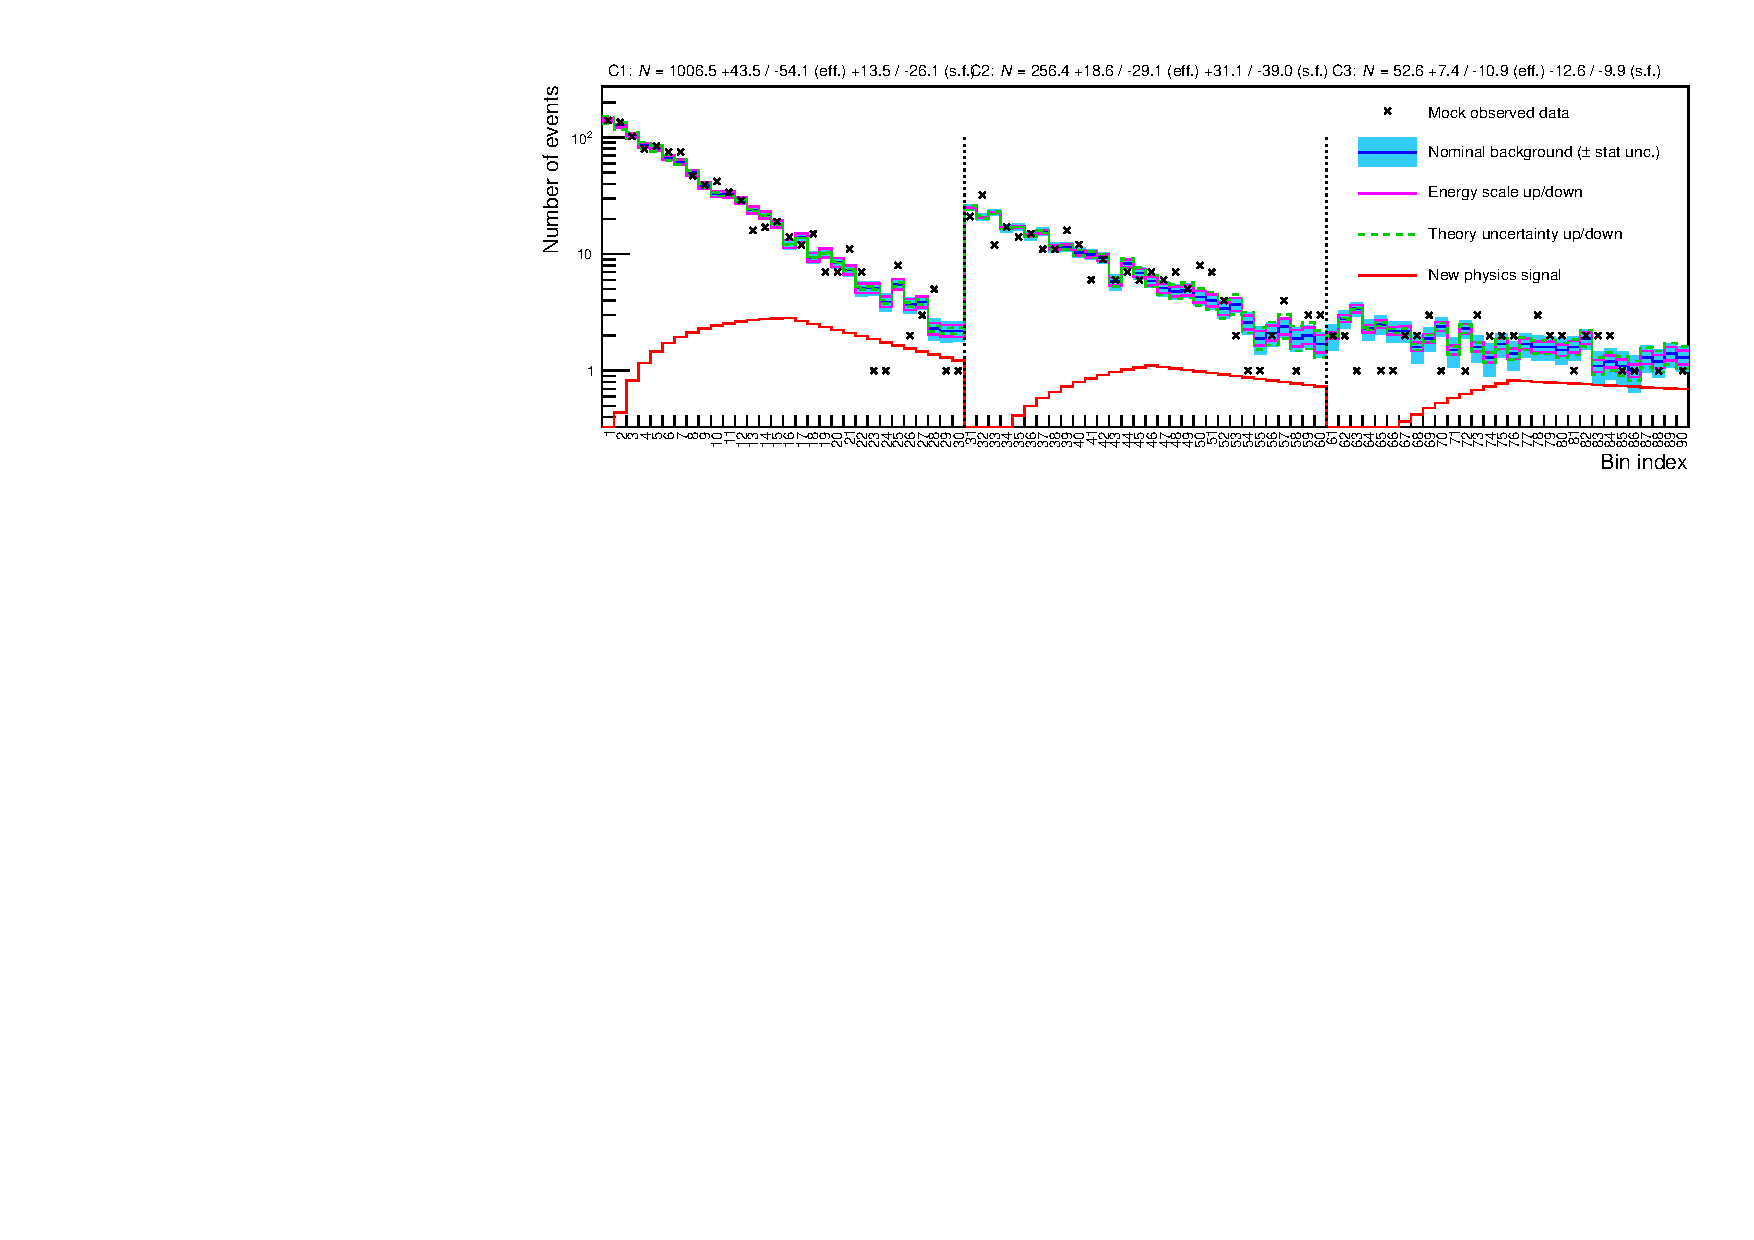
\includegraphics[width=\textwidth]{figures/t}
\end{center}
\caption{Toy search for new physics. The search is performed across three event categories, each divided into 30 bins to make a total of 90 search regions. The nominal expected contribution in each bin from the
background and from the new physics signal is shown by the blue and red lines, respectively. The solid and dashed lines show the $\pm1\sigma$ correlated variation in each bin expected due to an experimental and theoretical
uncertainty while the blue shaded band shows the uncorrelated uncertainty in each bin due to limited Monte Carlo simulation. The observed number of events in data in each bin is indicated by the black points.\textbf{TO BE UPDATED WITH FINAL TOY MODEL}}
\label{fig:toy}
\end{figure}


\subsection{Parameterization of backgrounds}

It is typical in experimental searches of this type to classify systematic uncertainties into three broad categories, namely; those which affect only the normalization of a given process, those which effect both the
`shape' or `distribution' of events of that process in addition to its normalization, and those which affect only a small number of bins or single bin in the distribution and are largely uncorrelated with the other
bins (eg uncertainties due to limited Monte Carlo simulation).

The expected (or nominal)\footnote{It should be noted that the expectation value for $n_{b,I}$ is \emph{not} necessarily the same as the mean value. For this reason, we typically refer
to this as the `nominal' value since it is the value attained when the elementary nuisance parameters are equal to their expectation values $\underline{\delta}=0$.} number of background events, due to a particular process, in a given bin ($I$) in Eqn~\ref{se:EL_SL} is denoted by
%
\begin{equation}
  n_{b,I}(\bm{\delta}) \equiv %\coloneqq
  f_{I}(\bm{\delta}) N(\bm{\delta}),
\end{equation}
%
where the process index ($k$) is suppressed here as we only have a single background process. The functions $N(\bm{\delta})$ and  $f_{I}(\bm{\delta})$ are is the total number of expected events for that process in a particular
category and the fraction of those events expected in bin $I$, respectively, for a specified value of $\bm{\delta}$. Often, these functions are not known exactly and some interpolation is performed between known
values of $n_{I}$ at certain values of $\bm{\delta}$. For each uncertainty, $j$, which affect the fractions, $f_{I}$, a number of different interpolation schemes exist. One common method however is to interpolate between
three distribution templates representing three values of $\delta_{j}$. Typically, these are for $\delta_{j}=0$, the nominal value, and $\delta_{j}=\pm1$ representing the plus and minus $1\sigma$ variations due to that uncertainty.

The interpolation is given by
%
\begin{equation}
 f_{I}(\bm{\delta}) = f_{I}^{0}\cdot\frac{1}{F(\bm{\delta})} \prod_{j} p_{Ij}(\delta_{j}),
 \label{eqn:frac_function}
\end{equation}
%
where $f_{I}^{0}=f_{I}(\bm{\delta}=0)$ and $F(\bm{\delta})=\sum_{I}f_{I}(\bm{\delta})$ ensures that the fractions sum to 1. In our toy search, as there are three event categories,
there are three of these summations, each of which runs over the 30 bins of that category. The polynomial $p_{Ij}(\delta_{j})$ is chosen to be quadratic between values of $-1 \leq \delta_{j} \leq 1$
and linear outside that range such that,

\begin{equation}
 p_{Ij}(\delta_{j}) = \begin{dcases*}
 		\frac{1}{2} \delta_{j}(\delta_{j}-1) \kappa_{Ij}^{-}  -(\delta_{j}-1)(\delta_{j}+1) + \frac{1}{2}\delta_{j}(\delta_{j}+1)\kappa_{Ij}^{+} & for $|\delta_{j}|<1$ \\
        \left[ \frac{1}{2}(3\kappa_{Ij}^{+} + \kappa_{Ij}^{-})-2\right]\delta_{j} - \frac{1}{2}(\kappa_{Ij}^{+}+\kappa_{Ij}^{-})+2 & for $\delta_{j}>1$ \\
         \left[2-\frac{1}{2}(3\kappa_{Ij}^{-} + \kappa_{Ij}^{+})\right]\delta_{j} - \frac{1}{2}(\kappa_{Ij}^{+}+\kappa_{Ij}^{-})+2 & for $\delta_{j}<-1$ \\
    \end{dcases*}
\end{equation}

The values of $\kappa_{Ij}^{-}$ and $\kappa_{Ij}^{+}$ are understood to be determined using the ratios of the template for a $-1\sigma$ variation to the nominal one and the $+1\sigma$
variation to the nominal one, respectively. The choice of using a quadratic interpolation and linear extrapolation is to avoid assuming to large a variation beyond the known
values\footnote{The validity of this interpolation scheme can (and frequently is) tested by comparing the interpolation to templates for additional, known values of $f_{I}$ for $\delta_{j}$ values other than $0,-1$ and $1$.}.

For uncertainties which directly modify the expected number of events $n_{i}$ of distribution, an exponent interpolation is used as the parameterization.
This is advantageous since the number of events, in any given bin, for this process is always greater than 0 for any value of $\delta_{j}$. For a relative uncertainty $\epsilon_{Ij}$, the fraction varies as
%
\begin{equation}
 \frac{n_{b,I}(\bm{\delta})}{n_{b,I}^{0}}  =  \prod_{j} (1+\epsilon_{Ij})^{\delta_{j}}.
  \label{eqn:bin_function}
\end{equation}
%
This is most common in the scenario where a limited number of Monte Carlo simulation events are used to determine the value of $n_{b,I}^{0}$
and hence some uncertainty is associated. As these uncertainties will be uncorrelated between bins of the distributions, most of the terms $\epsilon_{Ij}$ will be 0.

Systematic uncertainties which only affect the overall normalization, are also interpolated using exponent functions,
%
\begin{equation}
 N(\bm{\delta})  =   N^{0} \cdot \prod_{j} (1+K_{j})^{\delta_{j}},
 \label{eqn:norm_function}
\end{equation}
%
where $N^{0} = N(\bm{\delta}=0)$ and $j$ runs over the elementary nuisance parameters.  A simple extension to this arises if the uncertainty is `asymmetric', as in our toy search;
the value of $K_{j}$ is set to $K^{+}_{j}$ for $\delta_{j}\geq0$ and to $K^{-}_{j}$ for $\delta_{j} < 0$. Furthermore, any uncertainty which affects both the
shape and the normalization can be incorporated by including terms such as those in Eqn~\ref{eqn:frac_function} in addition to one of these normalization terms.
In our toy search, there will be a separate $N(\bm{\delta})$ term for each category which provides the total expected background rate summing over the 30 bins of that category.

Combining Eqns~\ref{eqn:frac_function},~\ref{eqn:bin_function} and~\ref{eqn:norm_function} yields the full parameterization,
%
\begin{equation}
 n_{b,I}(\bm{\delta}) = N^{0}\cdot \prod_{j}(1+K_{j})^{\delta_{j}} \cdot f^{0}_{I} \cdot\frac{1}{F(\bm{\delta})} \prod_{j} p_{Ij}(\delta_{j}) \cdot \prod_{j} (1+\epsilon_{Ij}\delta_{j}).
\label{eqn:expt_param}
\end{equation}

As already mentioned, a typical search for new physics will have contributions from multiple background processes, each with their own associated systematic uncertainties.
Only by summing over all of these backgrounds (i.e $n_{b,I}=\sum_{p}n_{b,p,I}$ for different background processes $p$) is the likelihood fully specified.


\subsection{Validation of the simplified likelihood}

Using our toy search, we compare the experimental and simplified likelihoods. \fxnote{Do we want a whole separate section for this after setting up the toy? We can compare 1. distributions (1D and 2D), 2. frequentist (profiled) and Bayesian (marginalised) likelihoods.}

Figure~\ref{fig:distributions} shows a comparison of the distribution of $\hat{n}_{i}$, for three of the bins, $i=4,50$ and $86$, between the experimental setup and the simplified one.
We constructed 100,000 pseudo-datasets by taking random values $\underline{\hat{\delta}}$, generated according to $\pi(\bm{\delta})$, and evaluating
$n_{b,I}(\hat{\bm{\delta}})$ for each dataset according to the Eqn~\ref{eqn:expt_param}. The black points show the projection of these toy datasets onto each bin index. The green line shows the
distribution of $\hat{n}_{b,I}$ when $\hat{n}_{b,I} = a_{I}+b_{I}\hat{\theta}_{I}+c_{I}\hat{\theta}_{I}^{2}$  and $\hat{\theta}_{I}\sim\mathcal{N}(0,1)$. The simplified likelihood coefficients
$a_{I},~b_{I}$ and $c_{I}$ are determined from the first three moments, which are calculated from the pseudo-datasets, and the resulting quadratic form shown in the inset panels. Additionally, the distribution
assuming a linear form ($\hat{n}_{b,I} = m_{1,I}+\hat{\theta}_{I}\sqrt{m_{2,II}}$) is shown by the red line.

\begin{figure}%[hbt!]
  \centering
  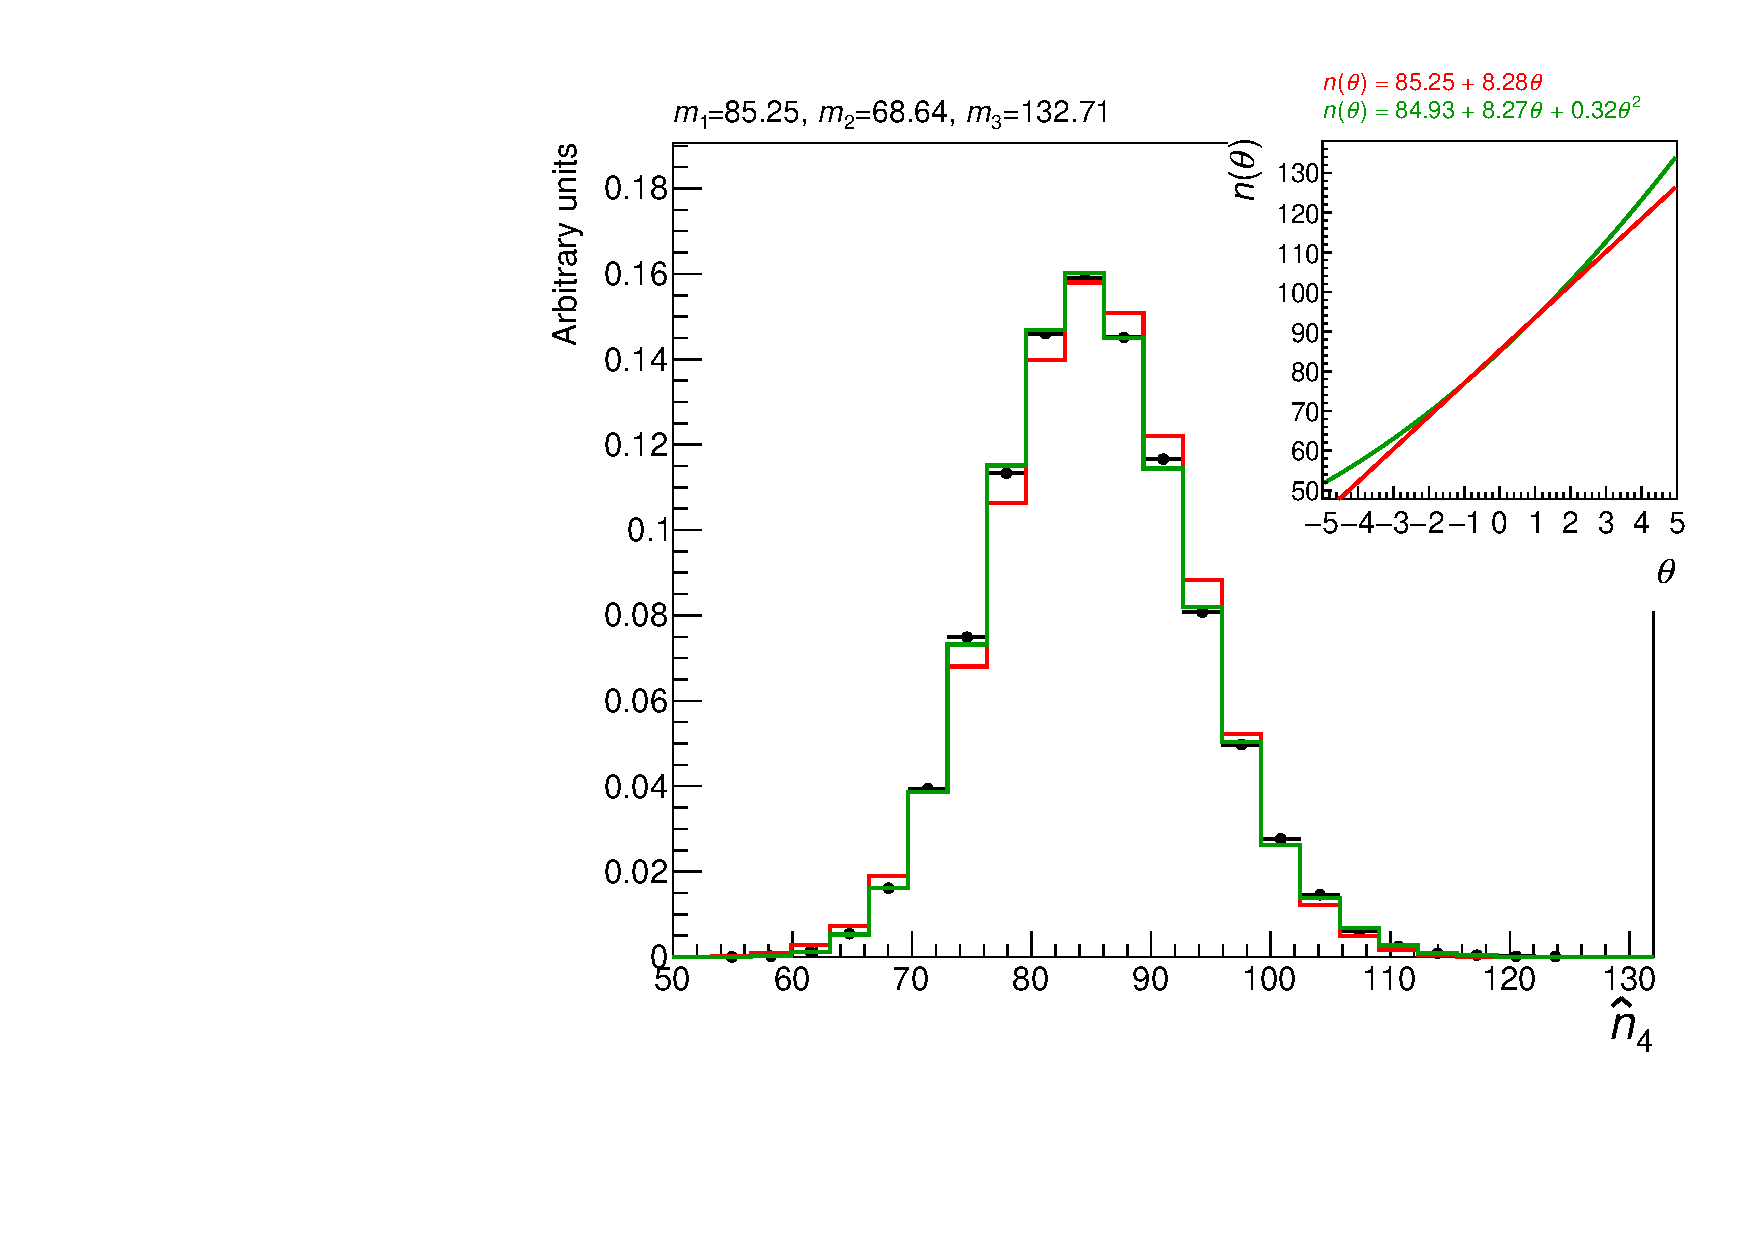
\includegraphics[width=0.32\textwidth]{figures/distribution_4}
  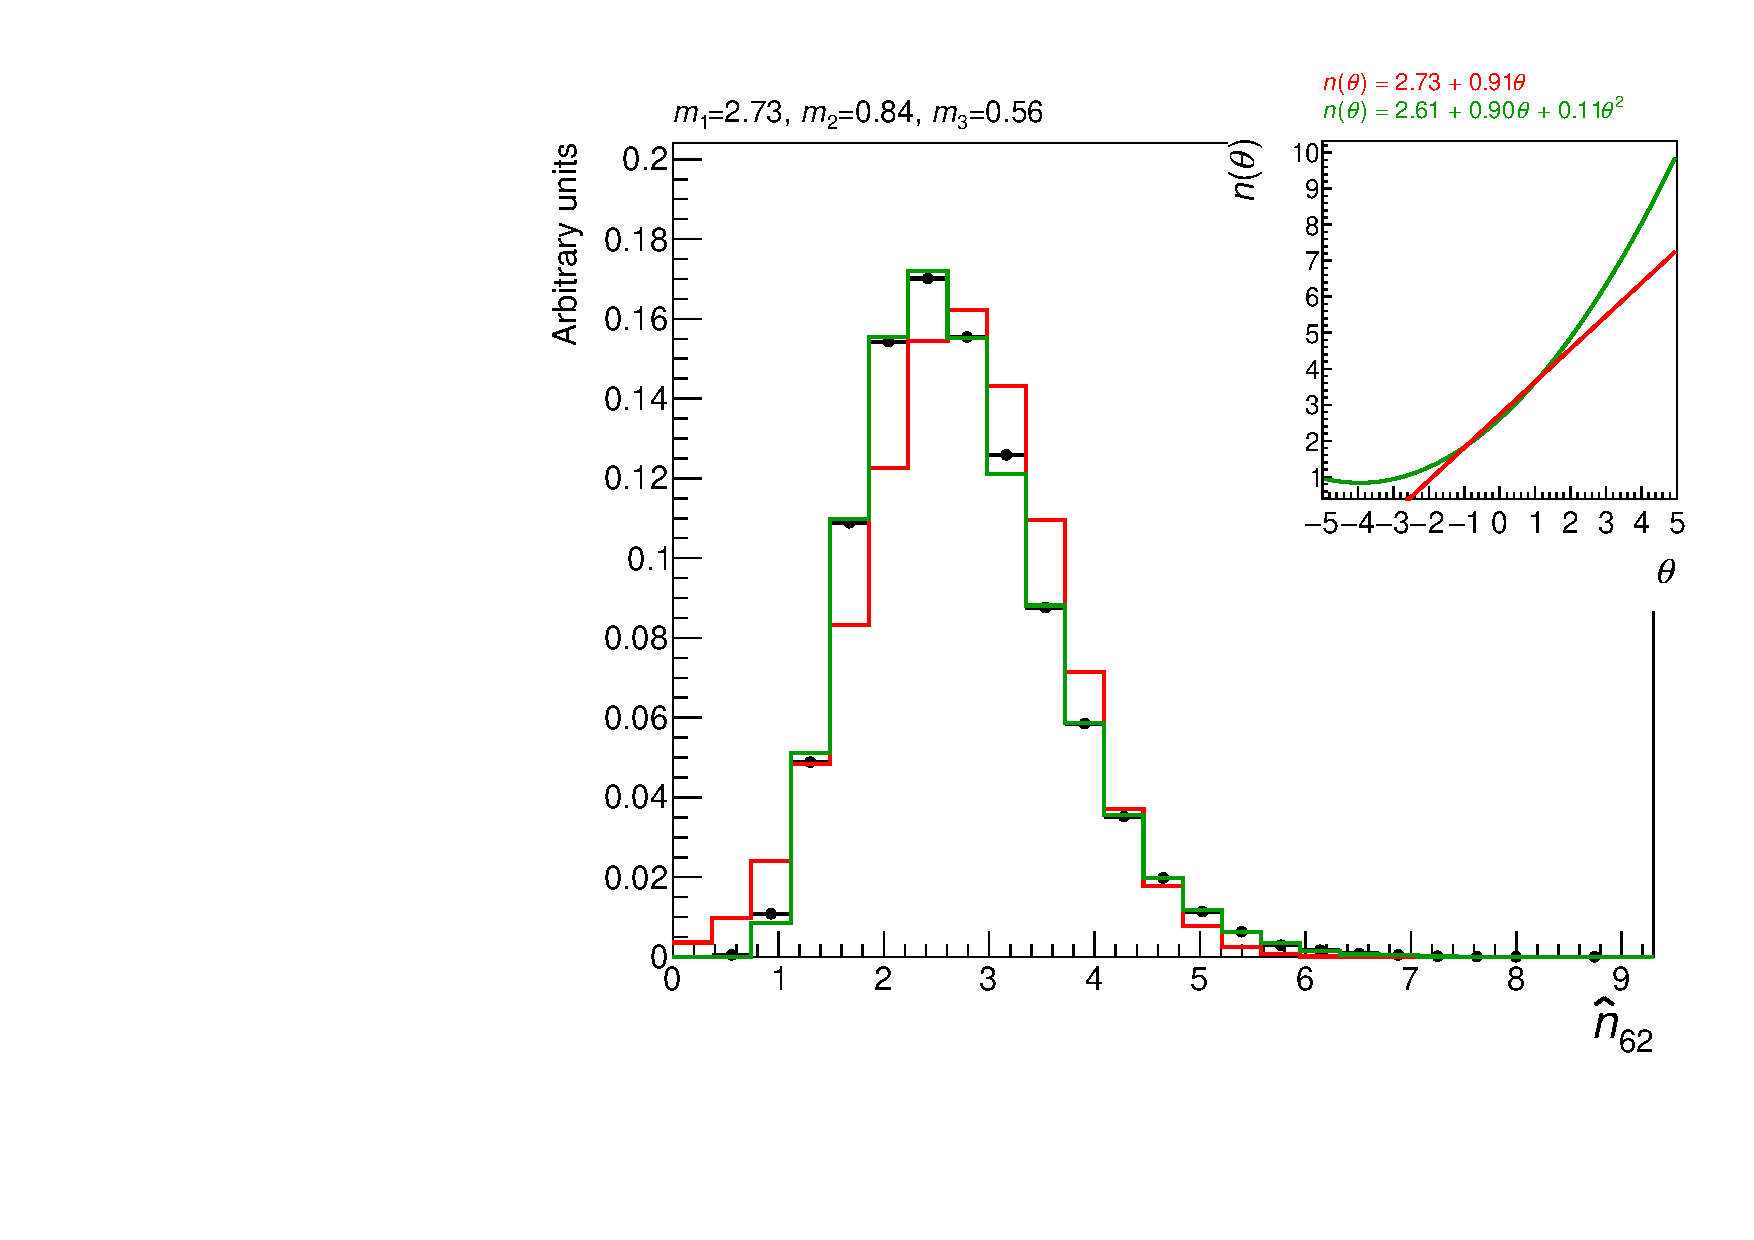
\includegraphics[width=0.32\textwidth]{figures/distribution_62}
  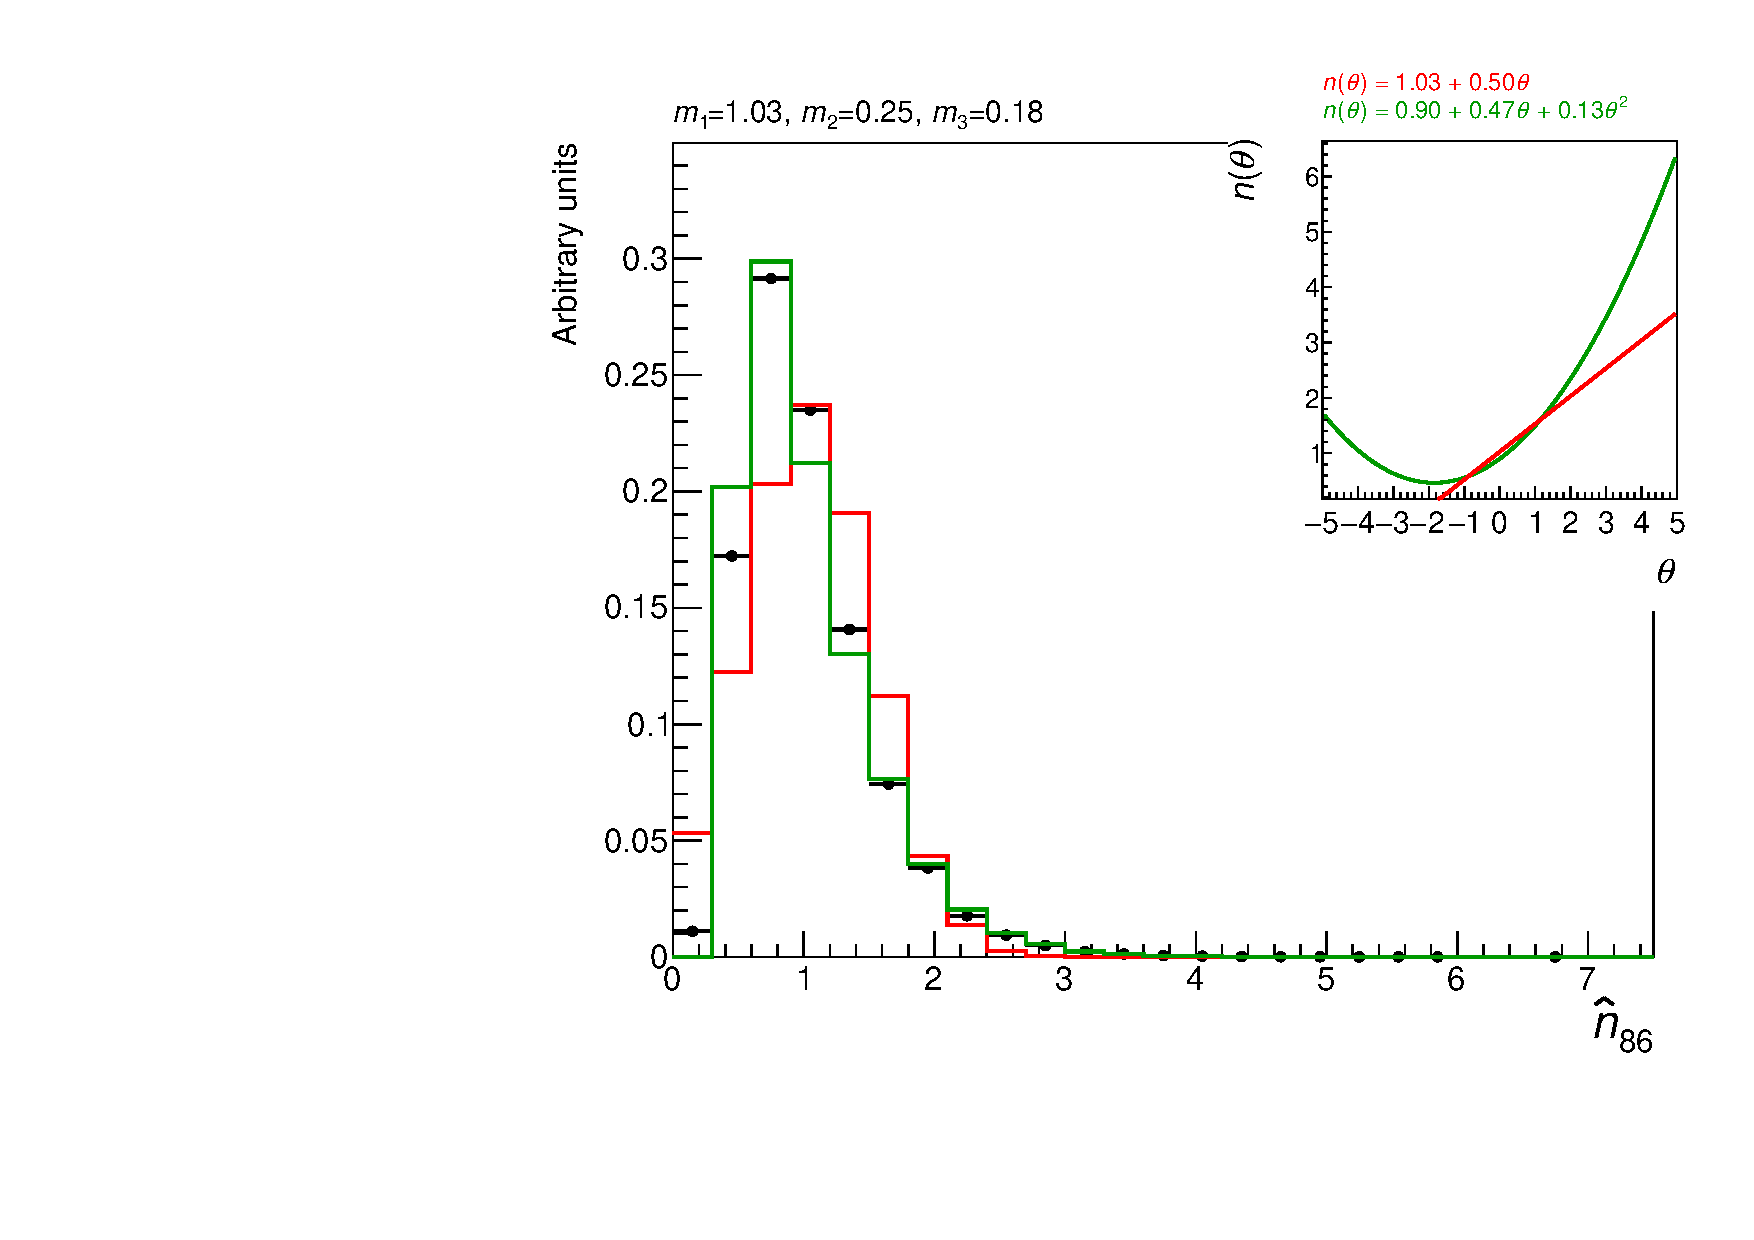
\includegraphics[width=0.32\textwidth]{figures/distribution_86}
  \caption{Distributions of $\hat{n}_{b,I}$ for $I=4$ (left), $I=62$ (center), and $I=86$ (right) in 100,000 pseudo-datasets generated from the experimental toy search (black points) as described in the text.
    % The error bars on the points indicate the statistical uncertainty from generating 10,000 toys.
    The functions $n_{I}(\theta_{I})$ assuming a quadratic form (green line), or
    a linear form (red line), are shown in the inset panels.  The distributions
    of $\hat{n}_{I}$ for the two cases (quadratic in green and linear in red)
    with $\hat{\theta}_{I}\sim\mathcal{N}(0,1)$ are shown.  }
  \label{fig:distributions}
\end{figure}

In the case where the skew of the distribution, defined as $m_{3,I}/(m_{2,II})^{\frac{3}{2}}$, is small,
both the linear and quadratic form produce a similar distribution as those from the pseudo-data.
Instead, for large values of the skew, the linear form leads to a shift of the peak in the distribution and overall poorer
agreement than the quadratic form. Moreover, in the quadratic form, the probability for $\hat{n}_{I}<0$
is much smaller when $n^{0}_{b,I}$ is small, as in the tails of the distributions (eg bin $86$), compared to the linear form.


\begin{figure}%[hbt!]
  \centering
  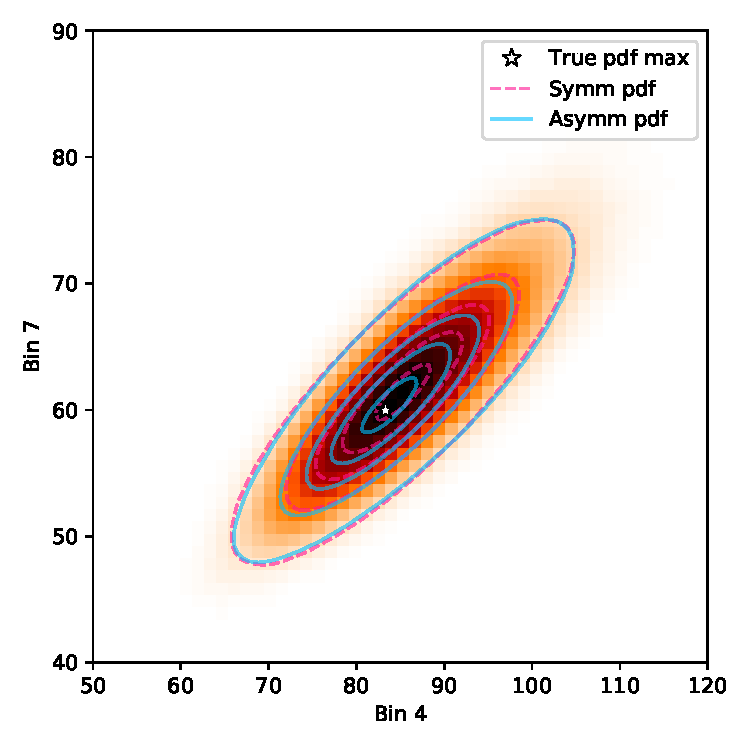
\includegraphics[width=0.45\textwidth]{figures/corr-4-7}
  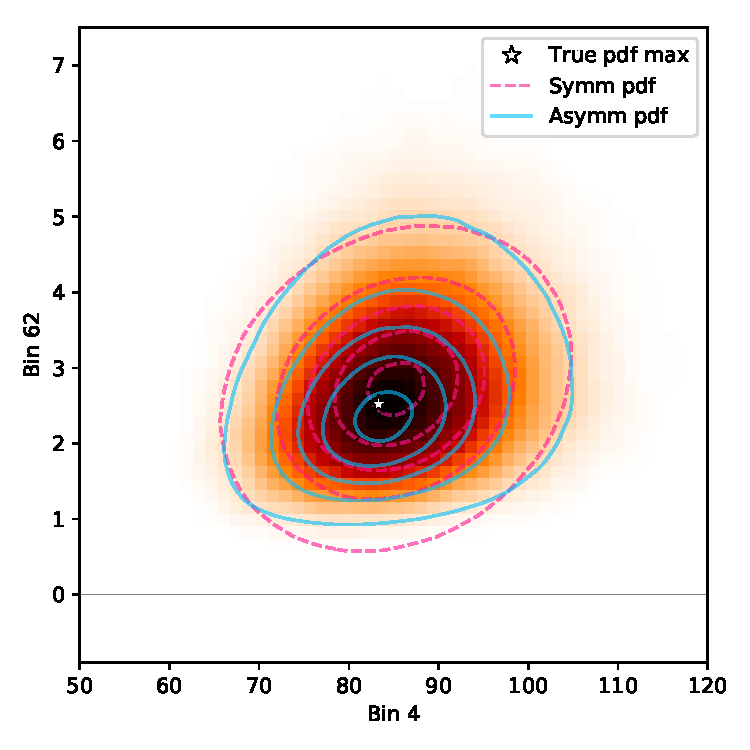
\includegraphics[width=0.45\textwidth]{figures/corr-4-62}\\
  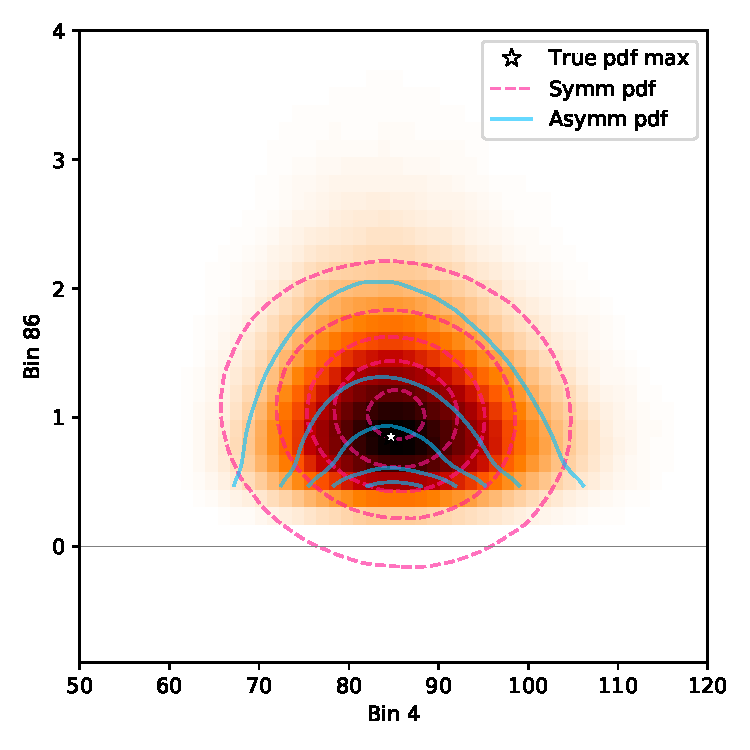
\includegraphics[width=0.45\textwidth]{figures/corr-4-86}
  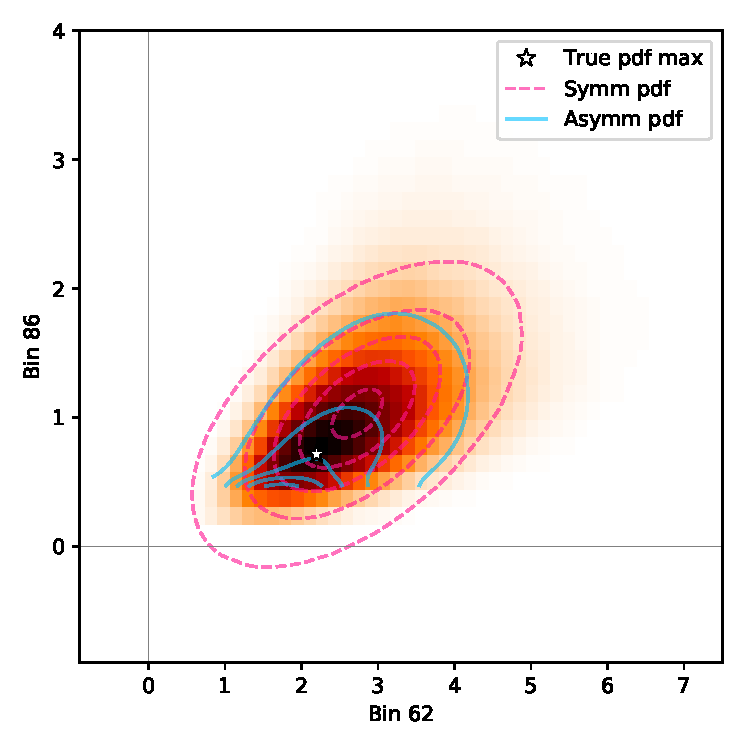
\includegraphics[width=0.45\textwidth]{figures/corr-62-86}
  \caption{2D distributions of $\hat{n}_{b,I}$ against $\hat{n}_{J}$ for
    % $I=4,J=62$ (left), $I=1,J=86$ (center) and $I=62,J=86$ (right)
    $I=4,J=7$ (top left), $I=4,J=62$ (top right), $I=4,J=86$ (bottom left), and
    $I=62,J=86$ (bottom right) in pseudo-datasets generated from the
    experimental toy search (black points) as described in the text. The
    background heat map is generated from 100,000 samples from the true toy
    model, the dashed pink countours from the linear SL form, and the solid
    light-blue contours from the quadratic SL form. In the pair of
    high-statistics bins in the top-left plot, clear agreement is seen between
    the linear and quadratic SL forms; in the top-right, deviations start to
    appear, and in the low-statistics bin~$J=86$ of the bottom plot the
    asymmetry is seen to become very significant, and the linear SL form has a
    significant probability density fraction in the negative-yield region.}
  \label{fig:distributions2d}
\end{figure}

In Figure~\ref{fig:distributions2d} 2D projections of the background
distributions are shown between four pairs of signal-region bins: bin pair
$(4,7)$ shows a projection for high-statistics bins where both the linear and
quadratic forms of the SL agree closely with the true distribution; the true
distribution in $(4,62)$ starts to display deviations from the multivariate
normal approximation which are well captured by the quadratic approximation; and
in the bottom pair of plots with bins~4 and~62 joint with the low-statistics
bin~86, the proximity of the mean rate to zero induces a highly asymmetric
Poisson distribution which neither approximation can model well. In these last
two plots, it can be seen that the quadratic-order SL peaks at too low a value,
near a sudden cutoff also seen in Figure~\ref{fig:distributions}, while the
linear form peaks at too high a value.  Systematic relaxation of the
quadratic-form cutoff to more closely model the true pdf would require
evaluation of higher-order coefficients (and/or off-diagonal skew terms) and
hence higher moments of the experimental distributions.

An advantage of the quadratic form cutoff is that a strictly positive
approximate distribution can be guaranteed, while the linear form can have a
significant negative yield fraction as seen in the figures for bin~86. Sampling
from the linear SL form, e.g.~for likelihood marginalisation, requires that the
background rates be positive since they are propagated through the Poisson
distribution. The quadratic SL provides a controlled solution to this issue,
as opposed to \emph{ad hoc} methods like use of a log-normal distribution or
setting negative-rate samples to zero or an infinitessimal value: the toy model
linear approximation has a negative fraction of $\sim\!11.6\%$, while the
quadratic form has a negative fraction of exactly zero.


\fxfatal{WOLFGANG: Plots showing profile \& marginalisation upper-limit
  extractions between true, symm/linear, and asymm/quadratic forms}


\section{Construction and distribution of Simplified Likelihood data}

\fxfatal{Give an introduction to the experimental/stats issues in extraction of
  stable and consistent 2nd and 3rd order correlation moments. Note the
  necessity of cross-checking and sanity-checking moment estimates: covariances
  have previously been published which, due to numerical rounding issues, are
  singular and hence unusable.}

Figure~\ref{fig:SLConvergence} shows the RMS of the simplified likelihood
coefficients for the three bins, $i=4,50$ and $86$ relative to the values
determined from 100,000 pseudo-datasets.

\begin{figure}%[hbt!]
  \centering
  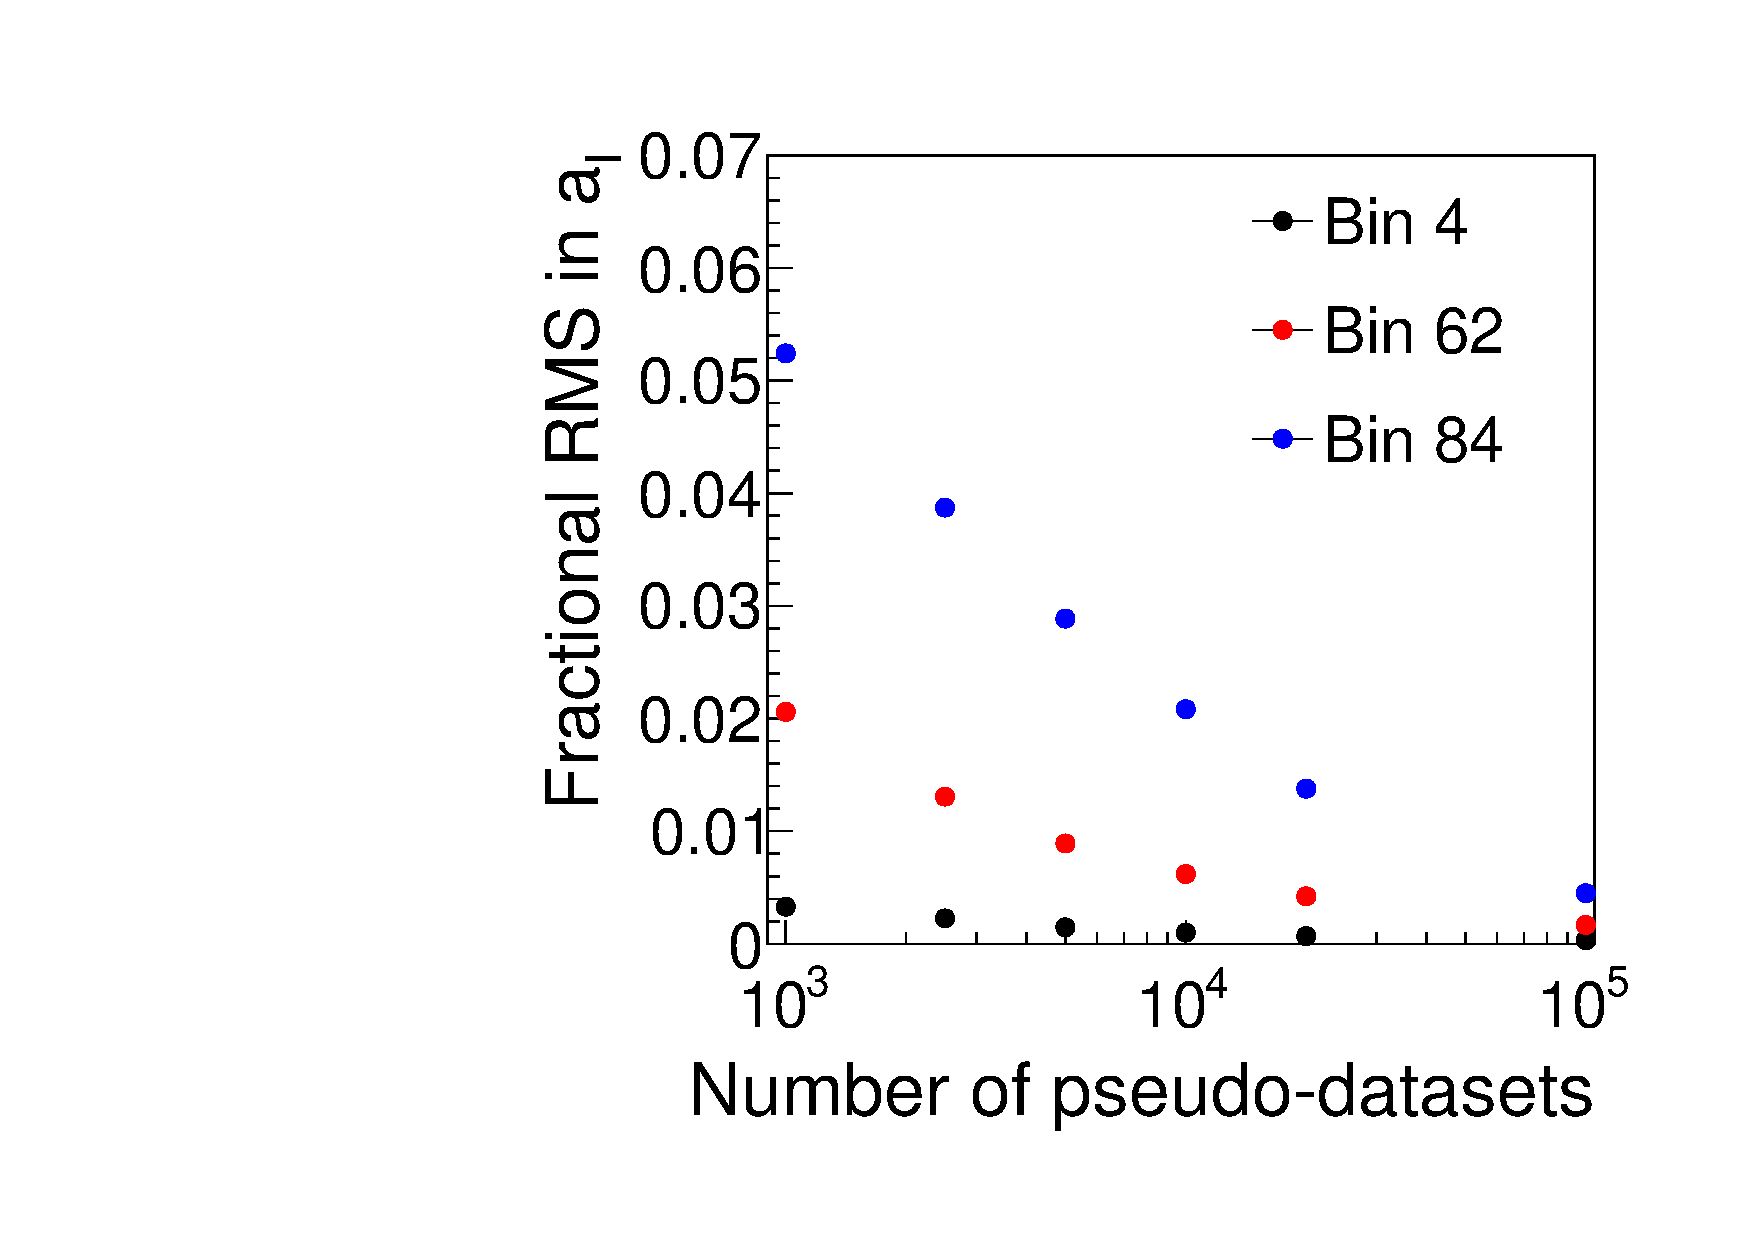
\includegraphics[width=0.32\textwidth]{figures/varAll_A}
  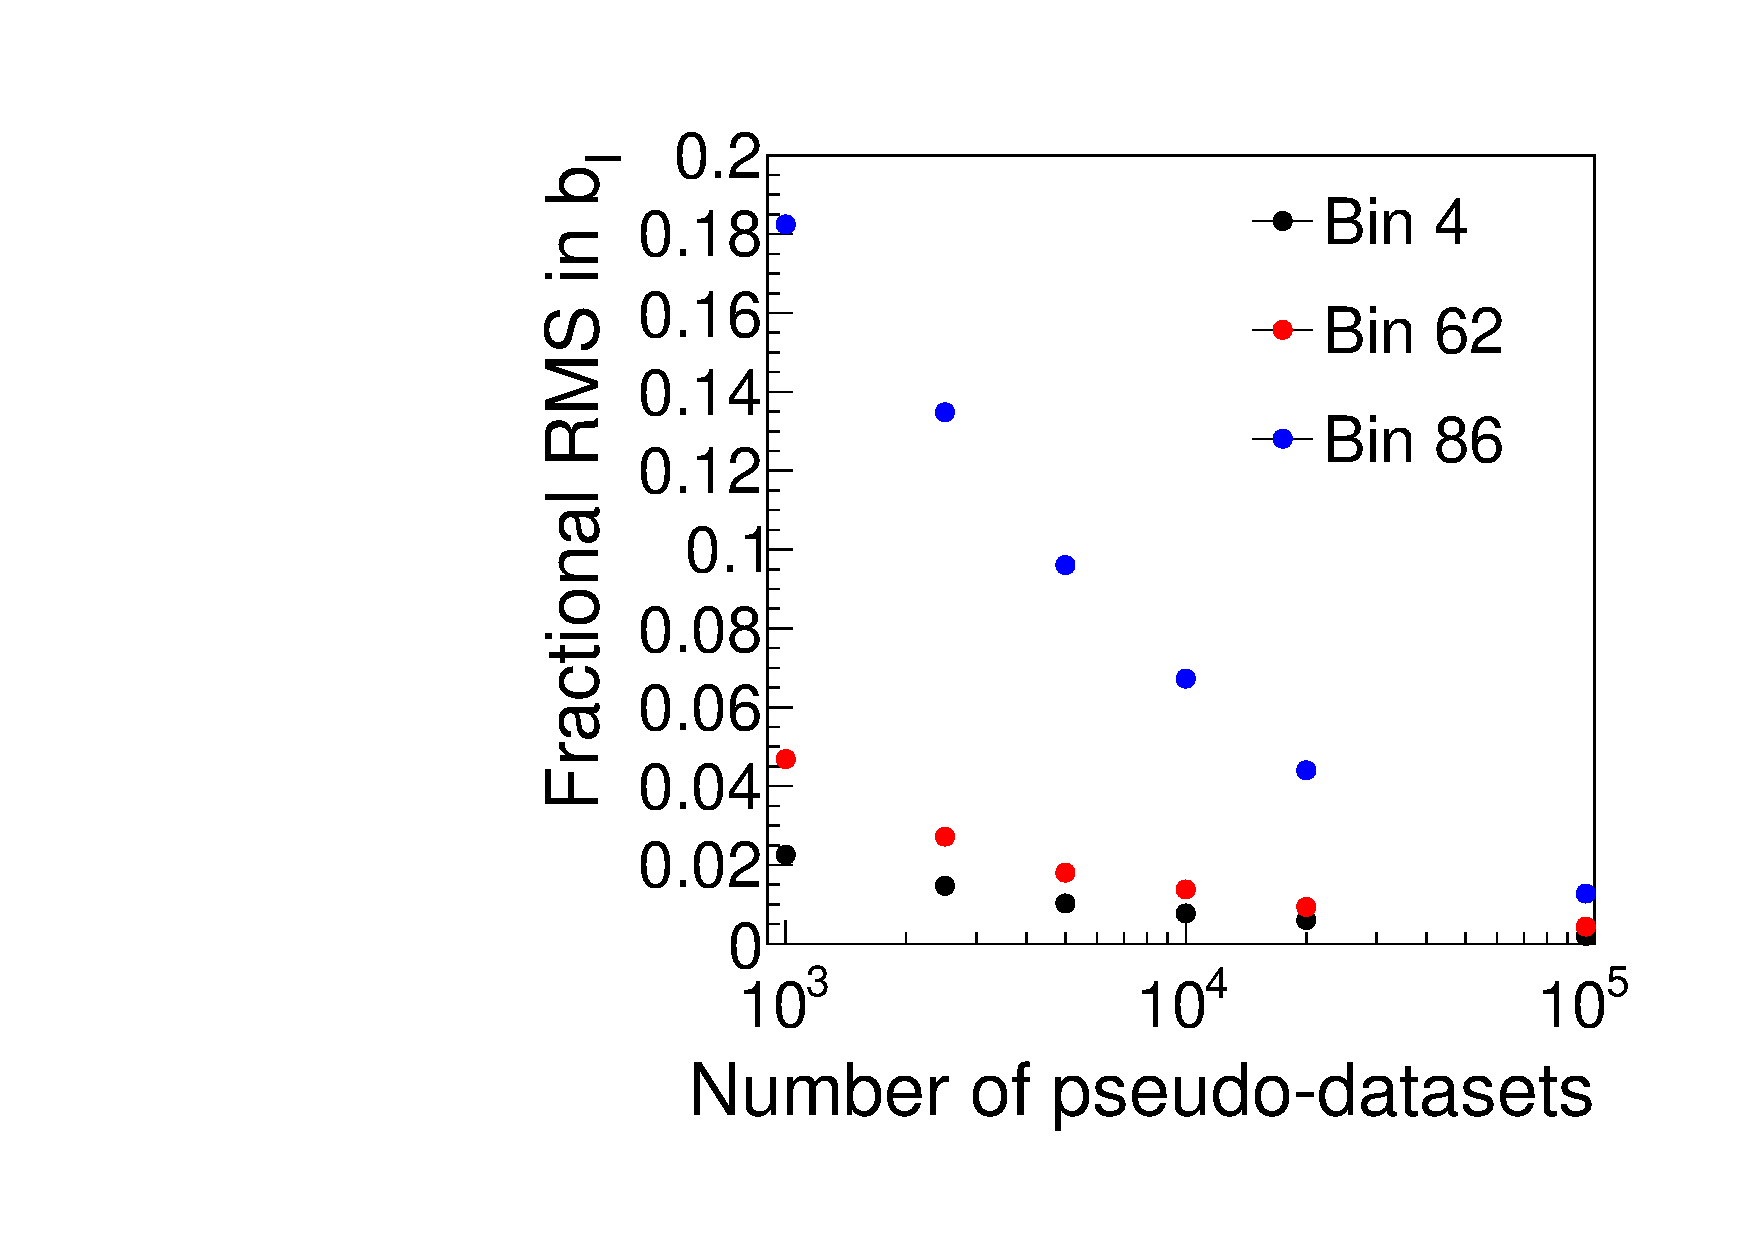
\includegraphics[width=0.32\textwidth]{figures/varAll_B}
  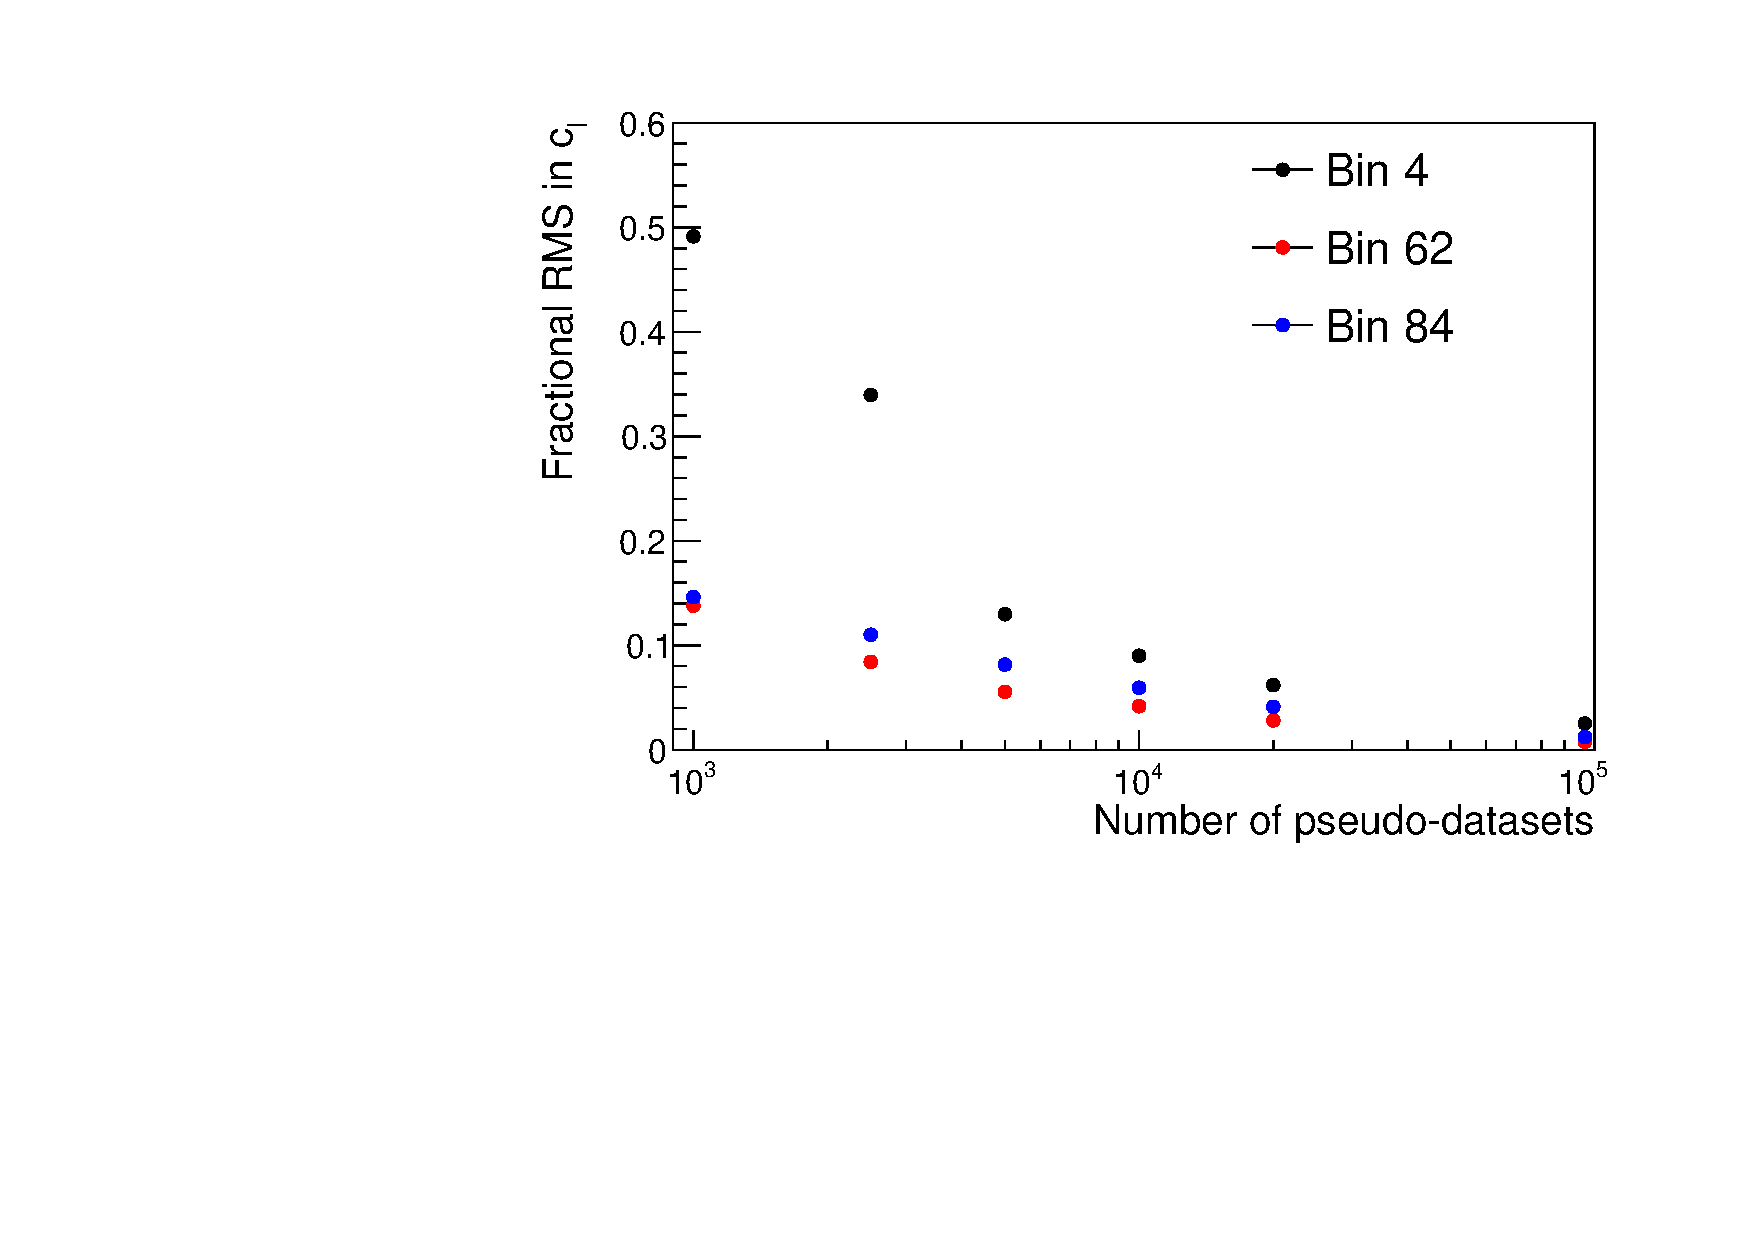
\includegraphics[width=0.32\textwidth]{figures/varAll_C}
  \caption{RMS of the simplfied likelihood coefficients relative to the mean
    coefficient value determined from 100,000 pseudo-datasets for $a_{I}$
    (left), $b_{I}$ (center), and $c_{I}$ (right). The distributions are shown
    for $I=4$ (black line), $I=62$ (red line) and $I=86$ (blue line).}
  \label{fig:SLConvergence}
\end{figure}

Key to the usefulness of any likelihood data for analysis reinterpretation is
the availability of that data in a standard format. For global fits, where tens
or hundreds of analyses may be used simultaneously, it is crucial that this
format be unambiguously parseable by algorithms without human assistance. A
standard location is also necessary, for which the obvious choice is the longstanding
HEP data repository, HepData~\cite{hepdata}.

Unfortunately, at present there is no standard semantic representation of second
order (i.e.~covariance) correlation data, let alone the third order ``skew''
information. At present a review of the correlation information in HepData and
on the experiments' analysis websites reveals a mixture of second-order data
presentation styles:
%
\begin{itemize}
\item 2D histograms of either covariance or correlation matrices. This has the
  difficulties that the convention used is not made clear (other than by
  inspection of the matrix diagonal), and without a structural association with
  a ``primary'' dataset of values/first moments it is impossible for computer
  codes to unambiguously construct the relevant likelihood. In the case of a
  normalised correlation representation cf.~$\rho$, the primary dataset must
  also provide the diagonal variances.
\item A breakdown by error-source, e.g. a series of labelled $\pm$ terms for
  each value in the primary dataset. From this, with some conventions (e.g.~a
  ''stat'' label to be a purely diagonal contribution, a ``lumi'' label to be
  100\% correlated across all bins, and all other labelled uncertainties treated
  as orthogonal) the correlation or covariance matrices can be constructed.
\item auxiliary files in arbitrary format: the \emph{ad hoc} nature of these
  makes them impossible to be handled by unsupervised algorithms. This includes
  2D histograms in ROOT data files, since variations in path structure and the
  ambiguity between covariance or correlation forms are an impeditment to
  automated use.
\end{itemize}

We offer two compatible proposals for this: augmentation of HepData table
headers to express relationships between tables, i.e.~identifying the second
(and third) moment data table associated with a primary dataset in a standard
and parseable fashion; and representation of SL covariance matrices in
error-source form, with each bin $I$ reporting $N$ different error sources of
value $\sqrt{m_{2,IJ}}$. Both would require some keyword standardisation: in the
first case to express the semantic type of a dataset and the relationships
between them, and in the second case to identify the diagonal error
term. Diagonal third-order moments can also be handled in both schemes,
trivially in the case of linked datasets, and by introduction of a new and
special ``skew'' label in the error-source scheme. Finally, a dataset annotation
would be required to indicate that the Poisson--Gaussian likelihood form
presented in this paper is the appropriate one to use, as opposed to e.g.~a pure
multivariate Gaussian cf.~$\chi^2$ testing.


\section*{Acknowledgements}

 This work has been initiated at the \textit{LHC Chapter II: The Run for New Physics} workshop held at IIP Natal.
 AB's work is supported by a Royal Society University Research Fellowship grant.
 SF's work is supported by the S\~ao Paulo Research Foundation (FAPESP) under grants \#2011/11973 and \#2014/21477-2.


\appendix

\section{The CLT at next-to-leading order}
\label{app:skew}




Let us show in a 1D example how the skew appears  in the asymptotic distribution. Consider $N$ independent centered nuisance parameters $\delta_j$ of variance $\sigma^2$ and third moment $\gamma$. Define \be Z=\frac{\sum_{j=1}^N \delta_j}{\sqrt{N}}\,.
\ee
The characteristic function of $Z$ is given by
\be
\varphi_Z(t)=\prod_{j=1}^N\varphi_{j}\left(\frac{t}{\sqrt{N}}\right),
\ee
where $\varphi_{j}(x) = {\bf E}[e^{ix\delta_{j}}]$.
 In the large $N$ limit, each individual characteristic function has the expansion
\be
\varphi_{j}\left(\frac{t}{\sqrt{N}}\right)= 1-\frac{\sigma^2 t^2}{2N}-i \frac{\gamma t^3}{6 N^{3/2}} +O\left(\frac{t^4}{N^2}\right)\,.
\ee
It follows that the full characteristic function $\varphi_Z$ then simplifies to
\be
\varphi_Z(t)=\exp\left(-\frac{\sigma^2 t^2}{2}-i \frac{\gamma t^3}{6 \sqrt{N}} +O\left(\frac{t^4}{N}\right)\right) \label{eq:CF_CLT}
 \ee
 This characteristic function is simple but has no exact inverse Fourier transform.


To go further, let us observe that the $Z$ random variable could in principle be written in terms of a normally distributed variable $\theta\sim {\cal N}(0,\sigma^2)$,
 with $Z=\phi(\theta)$ where $\phi$ is a mapping which is in general unknown.  At large $N$ however, we know that $Z$ tends to a normal distribution hence $\phi$ tends to the identity. Thus we can write $Z=\sqrt{N}\phi\left(\frac{\theta}{\sqrt{N}}\right)$ and Taylor expand for large $N$,
\be
Z=\theta+\frac{c}{2\sqrt{N}}\theta^2+O\left(\frac{1}{N}\right)\,.
\ee
Let us now compare the characteristic function of  this expansion to Eq.~\eqref{eq:CF_CLT}.
We find that the characteristic function is given by
\be
\varphi_Z(t)={\bf E} \left[ \mathrm{e}^{it \left(\theta+\frac{c}{2\sqrt{N}}\theta^2+O\left(\frac{1}{N}\right)\right)} \right]
%=\exp\left(-\frac{\sigma^2}{1-\frac{i c t}{\sqrt{n}}  +O(n^{-1})}\frac{t^2}{2}\right)
=\exp\left(-\frac{\sigma^2 t^2}{2}-i \frac{c t^3}{ 2 \sqrt{N}} +O\left(\frac{1}{N}\right)\right)
\label{eq:CF_exp}
\ee
after using the large $N$ expansion. This function matches Eq.~\eqref{eq:CF_CLT} for $c=\frac{\gamma}{3}$. Thus we have found the normal expansion provides a way to encode skewness in the large $N$ limit. Namely, we find that the $Z$ variable converges following
\be
Z\rightarrow \theta+\frac{\gamma}{3\sqrt{N}}\theta^2\,,\,\,N\rightarrow \infty  \quad \textrm{with } \quad \theta\sim{\cal N}(0,\sigma^2)\,.
\ee
When the quadratic term becomes negligible the distribution becomes symmetric, and we recover the usual CLT.
As expected, for finite $N$, we can see that  the support of $Z$ is not $\bf R$. For example for $\gamma>0$, we have
$Z > -3\sqrt{N}/4\gamma$.
%This normal expansion will be very useful in the simplified likelihood framework and
%will be extensively used in the following.

\section{Reference Code}
\label{sec:reference_code}

A reference implementation in Python code is provided in
\url{https://github.com/nucleosynthesis/SL-paper}.  This provides functions to
calculate the SL $a_I$, $b_I$, $c_I$, and $\rho_{IJ}$ coefficients, and an
\texttt{SLParams} class which computes these and applies them in combination
with observed and expected signal yields to calculate profile and marginal
likelihoods, log likelihood-ratios, and limit-setting test statistics. For
convergence efficiency, the profile likelihood computation makes use of the
gradients of the SL log-likelihood with respect to the signal strength $\mu$ and
nuisance parameters $\bm{\theta}$, which we reproduce here to assist independent
implementations:
%
\begin{align}
  \ln\! \big( L(\mu,\bm{\theta} )\pi(\bm{\theta}) \big) &=
  \sum_I^P \Big[ o_{I} \ln \left(\mu n_{s,I} + n_{I}(\theta_{I}) \right) - \left( \mu n_{s,I} + n_{b,I}(\theta_{I}) \right) - o_{I}! \Big]
  - \frac{1}{2} \bm{\theta}^\mathrm{T} \bm{\rho}^{-1} \bm{\theta} - \frac{P}{2} \ln 2\pi \\
  %
  \Rightarrow \qquad
  \frac{\mathrm{d}\ln L}{\mathrm{d}\mu} &= \sum_I^P \left( \frac{o_I}{\mu n_{s,I} + n_{b,I}(\theta_{I})} - 1 \right) \cdot \mu n_{s,I} \\
  %
  \frac{\mathrm{d}\ln L}{\mathrm{d}\theta_{\!A}} &= \left( \frac{o_A}{\mu n_{s,A} + n_{b,A}(\theta_{\!A}) } - 1 \right) \cdot \big( b_A + 2 c_A \theta_{\!A} \big) - \sum_I^P \rho_{\mspace{-1mu}AI}^{-1} \, \theta_I ~,
\label{eq:SL_LHC}
\end{align}
%
where $n_{b,I}(\theta_{I}) = a_{I} + b_{I}\theta_{I} + c_{I}\theta_{I}^{2}$.

%For simplicity, in our upcoming toy models, we will consider a single parameter-of-interest, the ratio of the observed to the predicted signal production cross-section $\mu=\sigma/\sigma_{\mathrm{TH}}$ (or `signal strength').
%This is very commonly used in experimental searches for some hypothetical new signal processes and demonstrates the simplified likelihood formalism without loss of generality.

\bibliographystyle{jhep}

\bibliography{biblio}

\end{document}
